\chapter{Related Work}\label{REL}

This chapter surveys the landscape in which Climatica was developed.
Section~\ref{REL_APPS} reviews existing climate data applications and identifies
the gap that Climatica addresses. Section~\ref{REL_WORLDCLIM} describes the
WorldClim dataset and the Virtual Semantic API on which the application depends.
Section~\ref{REL_SEMWEB} introduces the Semantic Web and Linked Data concepts
that underlie the API design. Section~\ref{REL_GEONAMES} describes GeoNames and
the Apache Solr search engine used for city search. Section~\ref{REL_WIKIDATA}
explains the role of Wikidata as a geographical knowledge base for reverse
geocoding. Section~\ref{REL_WL} describes the Walter-Lieth climatogram.

% * ─── 2.1 Existing Climate Data Applications ───────────────────────────────────
\section{A Survey of Climate Data Applications}\label{REL_APPS}

A number of web applications already offer access to climate and weather data.
The tools reviewed in this section were identified through web searches and
Google Scholar queries using terms such as \emph{climate data visualisation},
\emph{interactive climatogram}, and \emph{weather data explorer}. The selection
covers the most widely used publicly accessible tools that overlap with
Climatica's objectives, focusing on their intended audience, the data sources
they expose, and the interaction model they provide.

\subsection{ClimateCharts.net}\label{REL_APPS_CLIMATECHARTS}

ClimateCharts.net~\cite{climatecharts} is a browser-based tool that generates
Walter-Lieth climatograms for locations around the world. The user clicks a
point on an interactive map to select the nearest meteorological station, and
receives a climatogram together with basic monthly statistics. The interface is
clean and the output is immediately recognisable to anyone familiar with
classical climate classification.

The tool's main strength is its simplicity: a first-time user can obtain a
climatogram within seconds, with no registration or configuration required.
The chart is well-styled and the colour scheme adheres closely to the
traditional Walter-Lieth convention, making it easy to identify arid and humid
periods at a glance.

However, ClimateCharts.net is limited to a single view per location. There is
no mechanism for comparing two cities side by side, exploring how a location's
climate has changed across historical periods, or visualising the spatial
distribution of a climate variable across a region. Data are sourced from
meteorological station records, which means coverage is sparse in areas with
few weather stations --- large parts of Africa, Central Asia, and the Amazon
basin are poorly represented. The spatial resolution is inherently point-based
rather than raster-based, so interpolation between stations introduces
uncertainty in areas far from observation networks.

The interface of ClimateCharts.net is shown in Figure~\ref{fig:screenshot_climatecharts}.
\begin{figure}[t]
  \centering
  \subfigure[Map interface: the user clicks a location to select the nearest
  climate cell.]{
    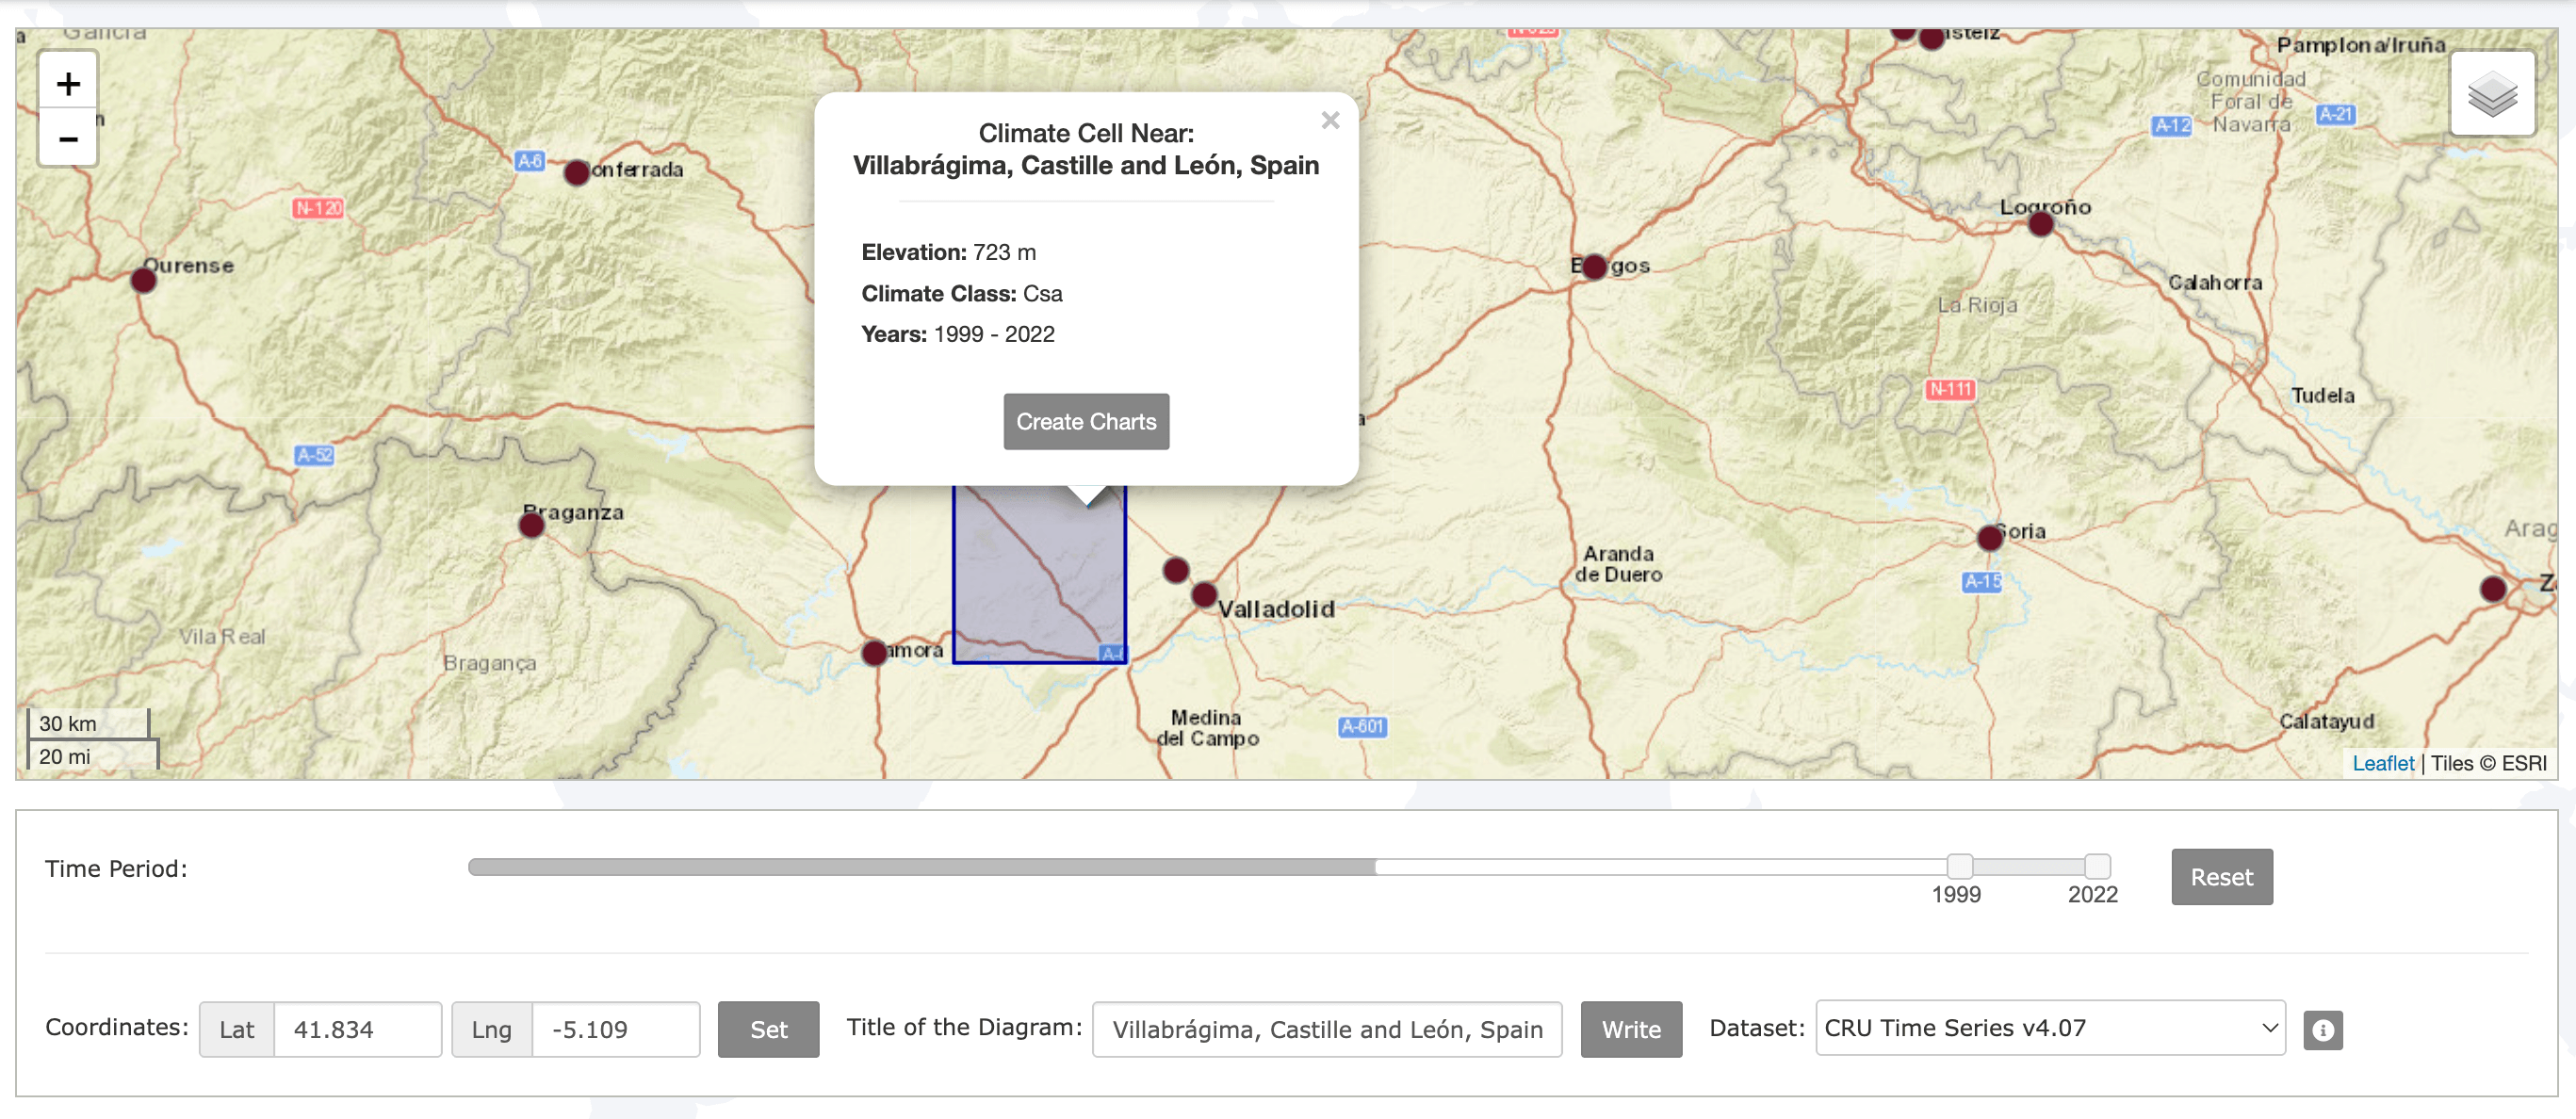
\includegraphics[width=0.9\textwidth]{Images/climatecharts-map.png}
  }
  \subfigure[Resulting Walter-Lieth climatogram with monthly data table.]{
    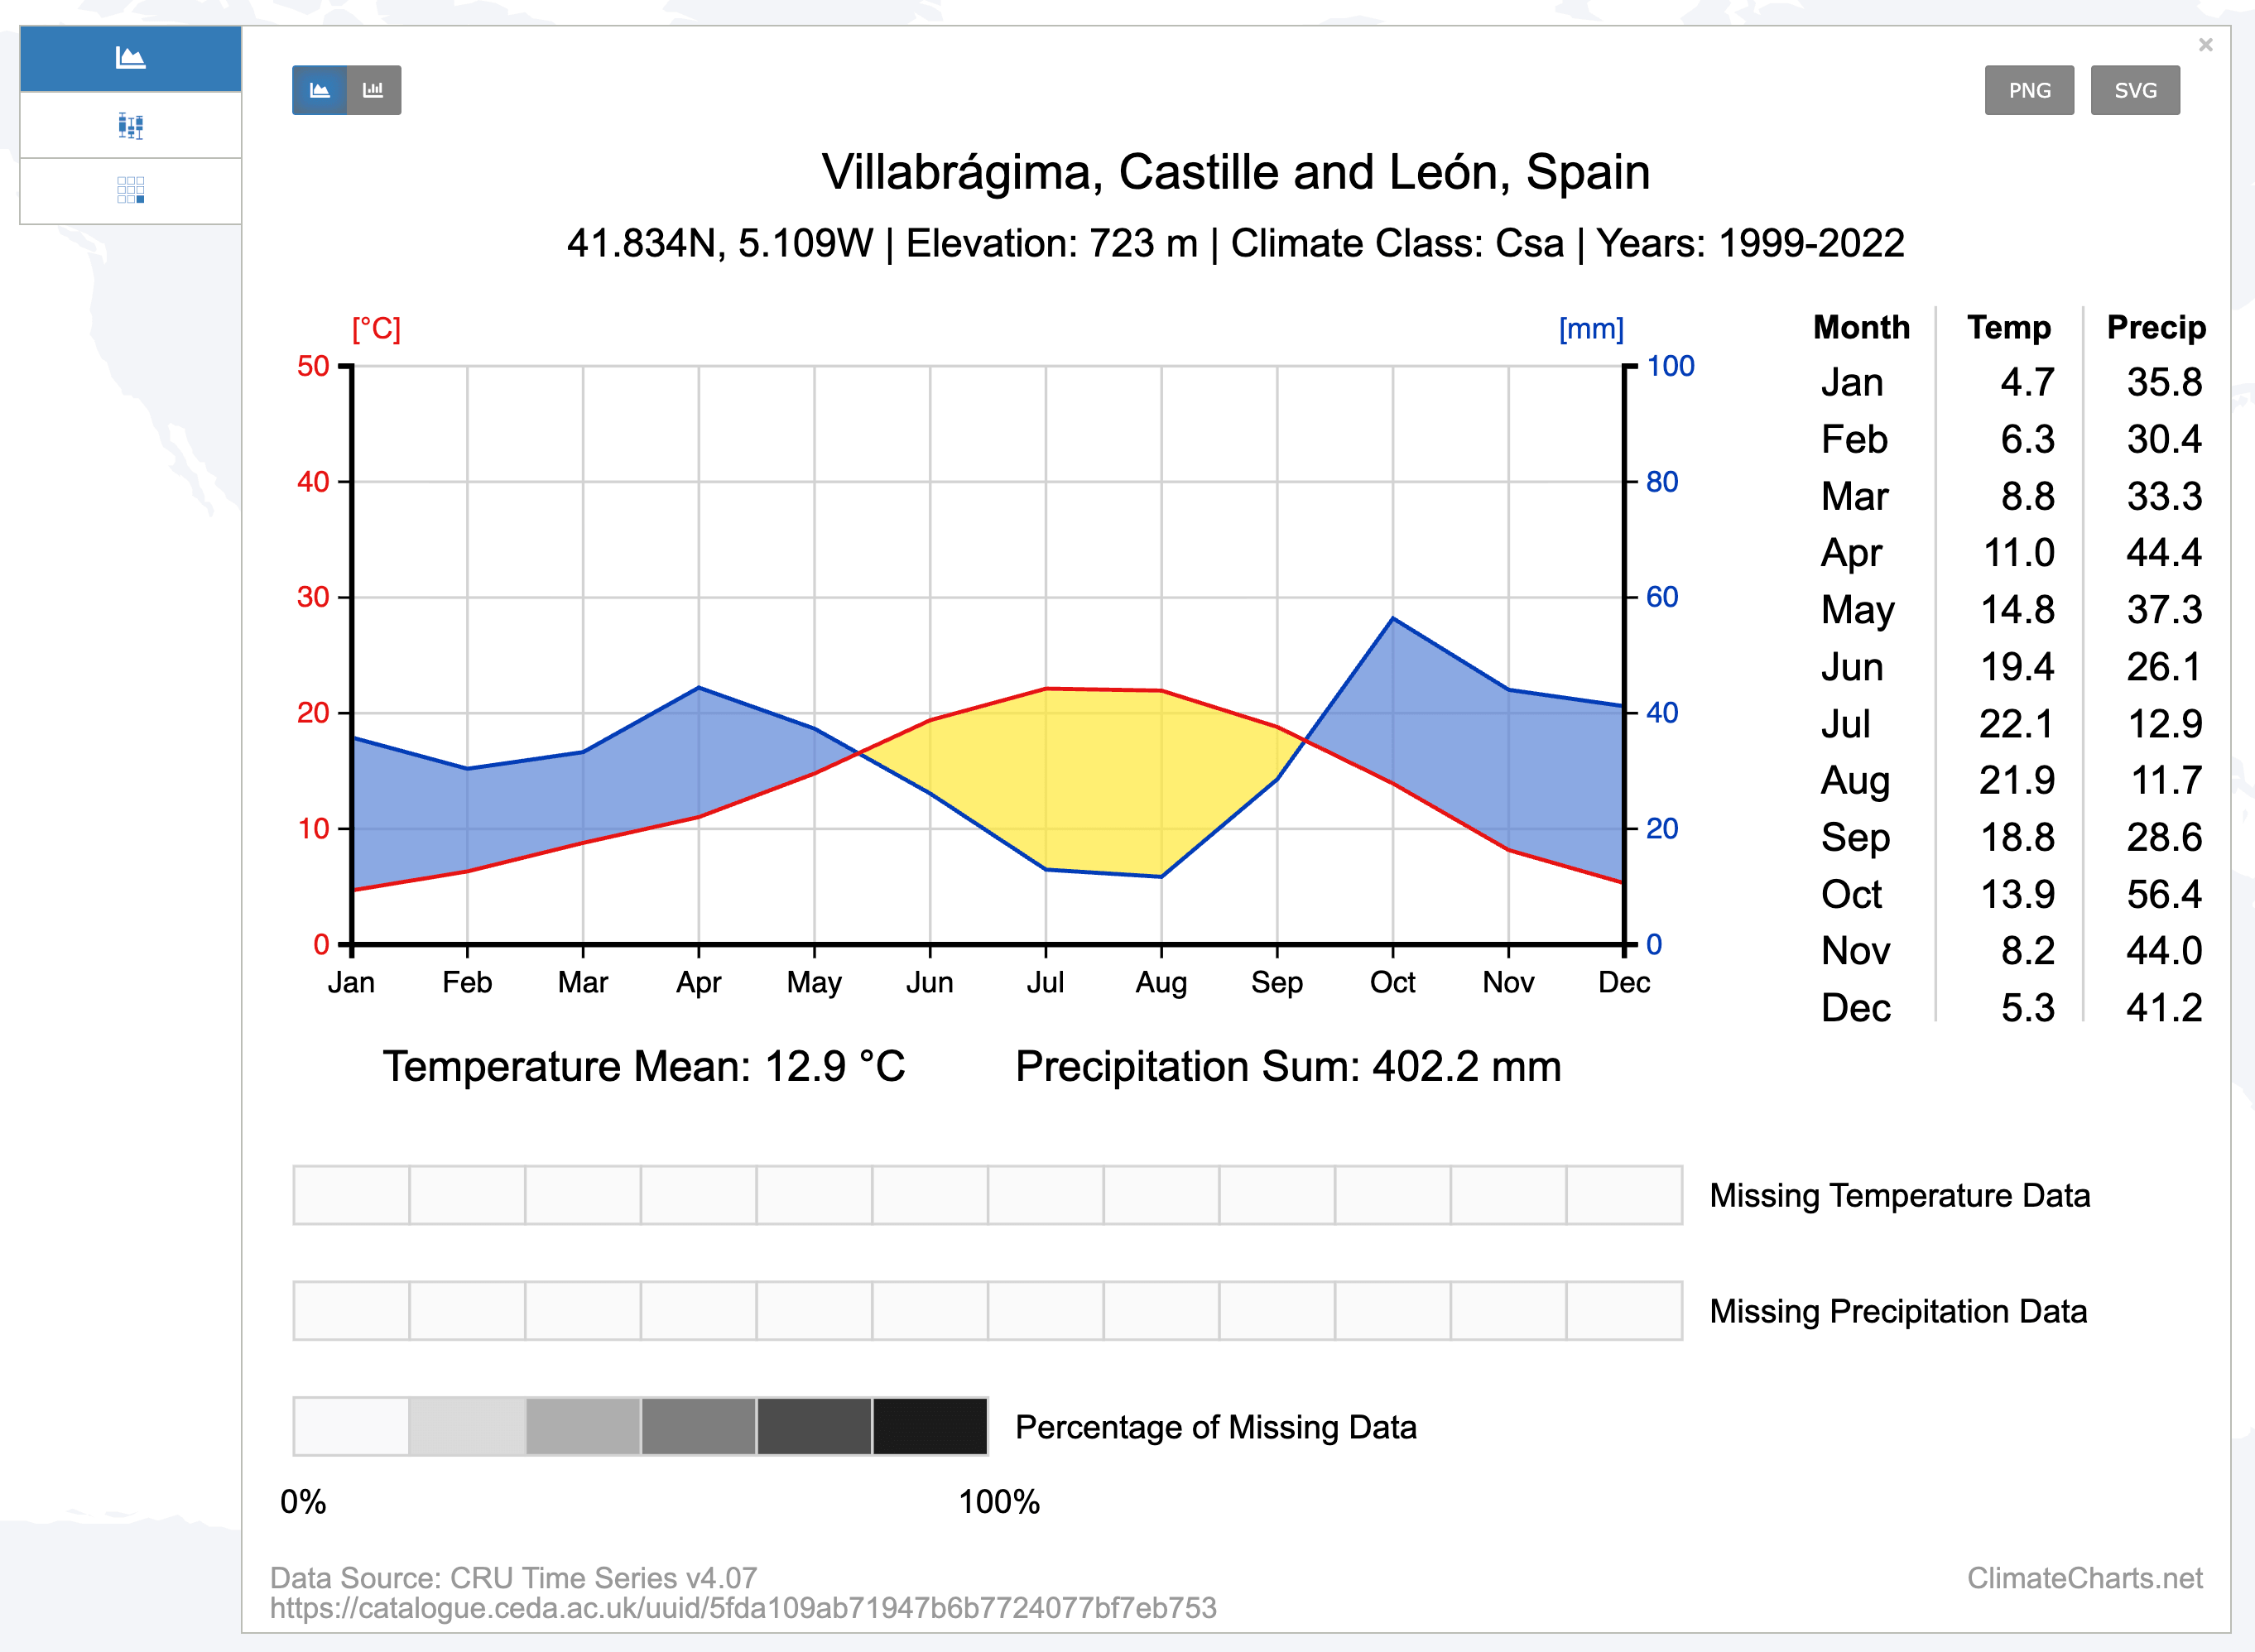
\includegraphics[width=0.9\textwidth]{Images/climatecharts-chart.png}
  }
  \caption{ClimateCharts.net interface. The tool produces clean Walter-Lieth
    climatograms but is limited to a single location view with no comparison or
  temporal exploration features.}
  \label{fig:screenshot_climatecharts}
\end{figure}

\subsection{Climate-Data.org}\label{REL_APPS_CLIMATEDATA}

Climate-Data.org~\cite{climatedataorg} provides climate statistics and
climatograms for thousands of cities worldwide. Each city page displays monthly
averages for temperature and precipitation alongside a pre-rendered diagram.
The site is primarily informational: data are presented as static charts and
tables with no interactive controls beyond city selection.

From a user-experience perspective, the interface can feel cluttered, with
advertising banners and navigation menus that are not immediately intuitive for
a first-time visitor. The data themselves are reliable --- the site draws on
established meteorological records --- but the presentation prioritises
comprehensiveness over clarity. A user who wants only to understand the broad
seasonal pattern of a location must scroll past a considerable amount of
supplementary content to find the chart.

The absence of comparative or temporal views means the site is not suited to
exploratory analysis. There is no way to ask questions such as ``how does the
summer in Valladolid compare to that in Kyiv?'' or ``has the dry season in this
city become longer over the past fifty years?''. The site does not expose a
public API, so its data cannot be consumed programmatically by third-party
applications. Furthermore, the temporal coverage is limited to a single climate
period (1991--2020), no Walter-Lieth climatogram is available, and the location
database covers only a subset of populated places --- many smaller settlements
are absent entirely.

Figure~\ref{fig:screenshot_climatedata} shows a typical city page from the site.
\begin{figure}[t]
  \centering
  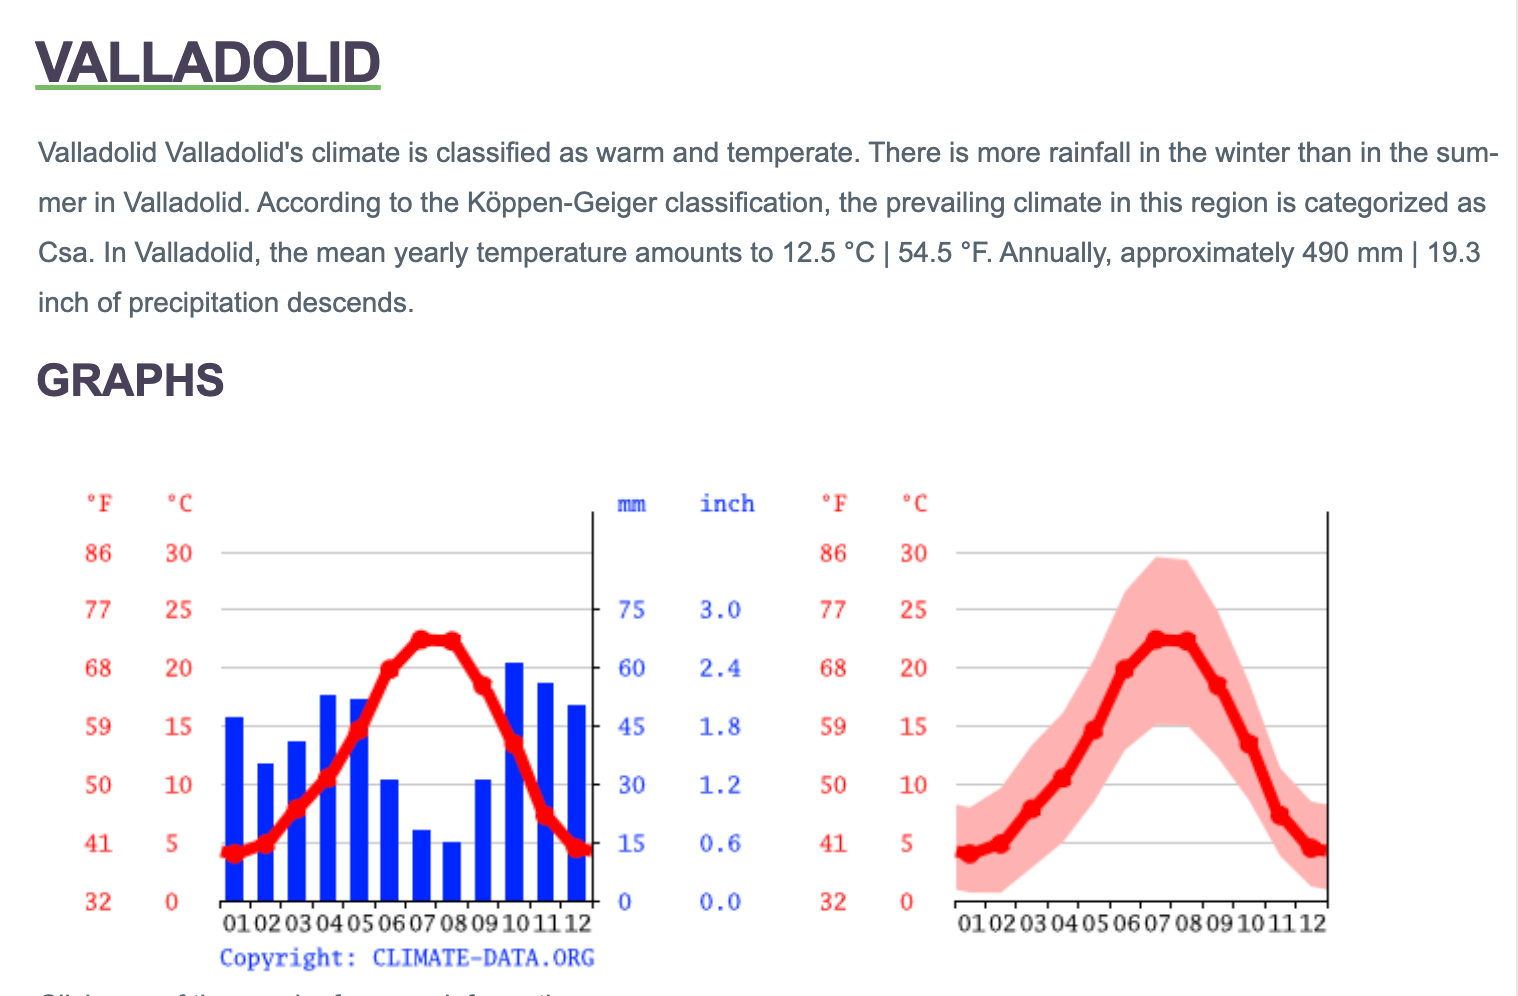
\includegraphics[width=0.9\textwidth]{Images/climatedata.png}
  \caption{Climate-Data.org city page. The static climatogram and data tables
    are embedded among advertising and navigation elements, making the interface
  feel cluttered for a user interested primarily in the chart.}
  \label{fig:screenshot_climatedata}
\end{figure}

\subsection{Meteoblue}\label{REL_APPS_METEOBLUE}

Meteoblue~\cite{meteoblue} is a commercial weather and climate platform that
offers high-resolution forecasts, historical reanalysis data, and climate
simulations. Its History and Climate module provides multi-decadal statistics
for any location, displaying average temperatures, precipitation, hot days,
cold nights, and wind speed on a single interactive chart. The platform is aimed
at a broad audience ranging from casual users planning holidays to professionals
in agriculture, aviation, and construction.

Compared to ClimateCharts.net and Climate-Data.org, Meteoblue provides
considerably more information per view: a single chart may overlay five or more
variables simultaneously, and the interface includes a Climate Comparison
feature that allows two locations to be placed side by side. In this respect,
Meteoblue overlaps with several of Climatica's objectives.

However, there are meaningful differences in scope and data source. Meteoblue
relies on ERA5T~\cite{hersbach2020era5}, a reanalysis dataset produced by the
European Centre for Medium-Range Weather Forecasts (ECMWF) that combines
observational data with numerical weather modelling. This makes it well suited
for recent weather reconstruction but less directly comparable with the
station-interpolated WorldClim surfaces that Climatica uses. Furthermore, the
density of information presented --- multiple overlapping lines, dual axes, and
a legend with five entries --- can be overwhelming for a first-time user who
simply wants to know whether July is dry or wet in a given city. Climatica takes
a different design choice: fewer variables per view, a cleaner visual hierarchy,
and a focus on the Walter-Lieth convention that many geography students and
educators already know.

Figure~\ref{fig:screenshot_meteoblue} shows the History and Climate module
for Valladolid.
\begin{figure}[t]
  \centering
  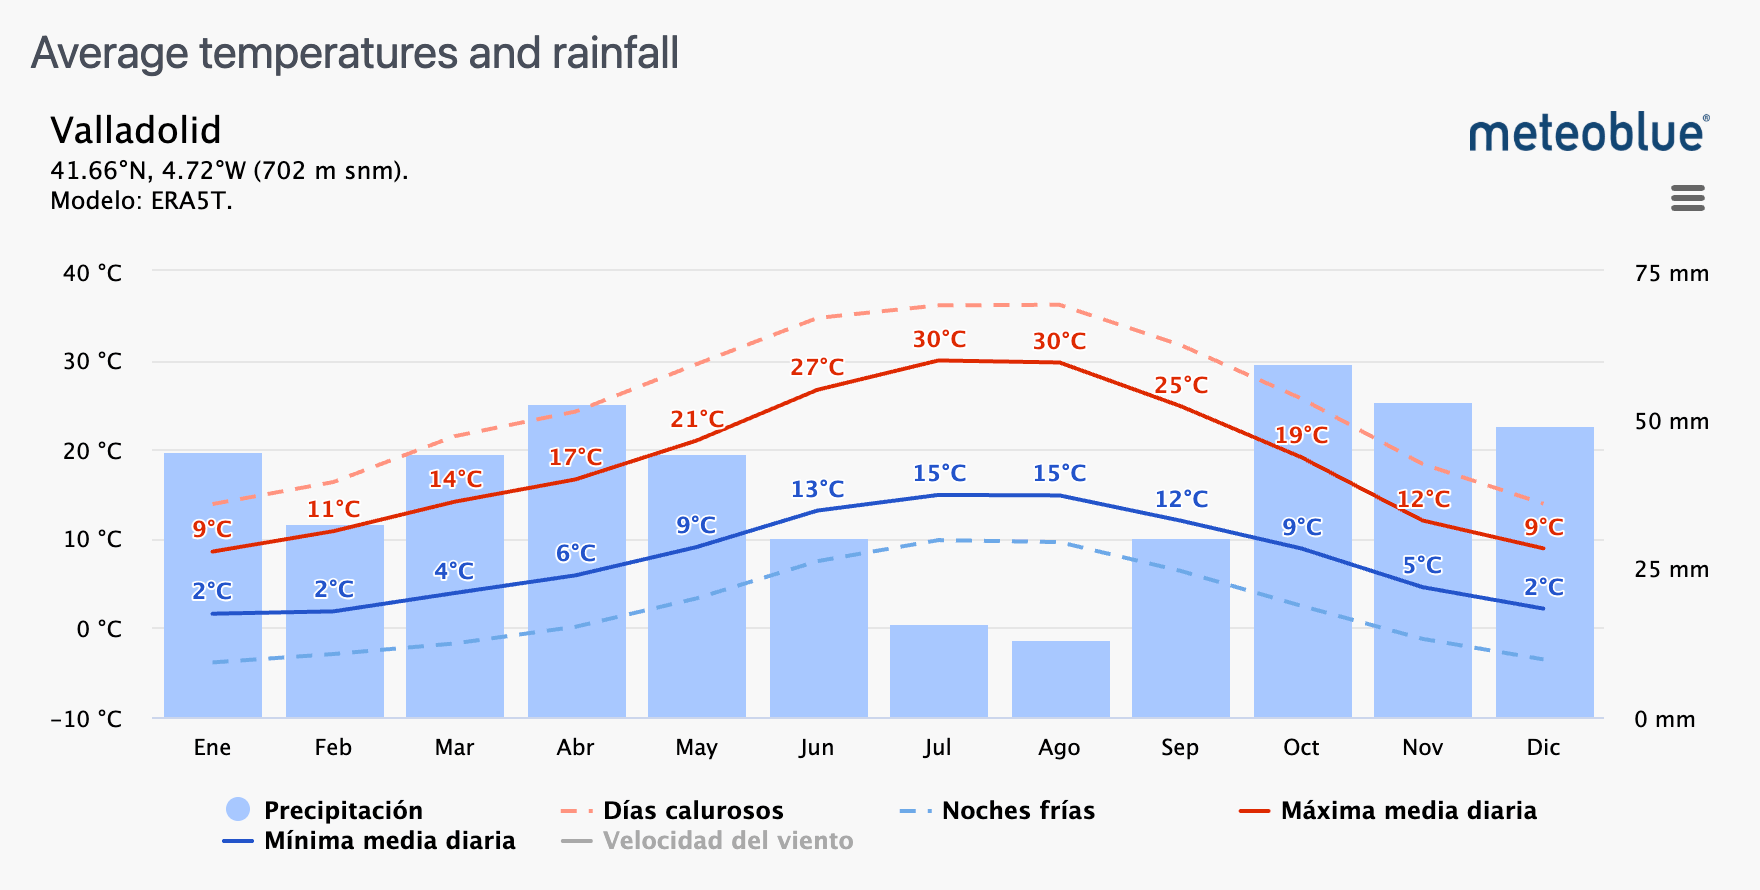
\includegraphics[width=0.9\textwidth]{Images/meteoblue.png}
  \caption{Meteoblue History and Climate module for Valladolid. The chart
    overlays five climate variables simultaneously and is backed by the ERA5T
    reanalysis dataset. The platform offers more data per view than
    ClimateCharts.net but targets a different audience and data source than
    Climatica.}
  \label{fig:screenshot_meteoblue}
\end{figure}

\subsection{NASA Giovanni}\label{REL_APPS_GIOVANNI}

NASA Giovanni~\cite{giovanni} (Geospatial Interactive Online Visualization ANd
aNalysis Infrastructure) is a web-based platform developed by NASA's Goddard
Earth Sciences Data and Information Services Center (GES DISC). It provides
access to a vast archive of satellite-derived geophysical data, including
surface temperature, precipitation, aerosol optical depth, and dozens of other
atmospheric and land-surface variables. The platform is designed for scientific
research and supports a wide range of analysis operations: time-series
extraction, area-averaged plots, spatial maps, correlation analyses, and
hovmöller diagrams, among others.

Giovanni's primary strength is the breadth and scientific rigour of its data
holdings. Variables are derived from well-validated satellite missions such as
MODIS, TRMM, and GPM, and the platform provides access to data spanning
multiple decades. The spatial coverage is global, and the temporal resolution
ranges from daily to monthly depending on the variable and mission.

However, Giovanni is clearly designed for atmospheric scientists and remote
sensing specialists. The workflow for retrieving data requires the user to
navigate a multi-step interface: select a variable from a hierarchical catalogue
of thousands of datasets, specify a spatial bounding box, choose a time range,
select an analysis type, and submit a processing job that may take several
minutes to complete. The results are returned as downloadable files or rendered
charts, but there is no interactive exploration mode in which a user can click a
city on a map and immediately see its climate profile. The platform is powerful
but has a steep learning curve that puts it out of reach for non-specialist
users.

The NASA Giovanni interface is shown in Figure~\ref{fig:screenshot_giovanni}.
\begin{figure}[t]
  \centering
  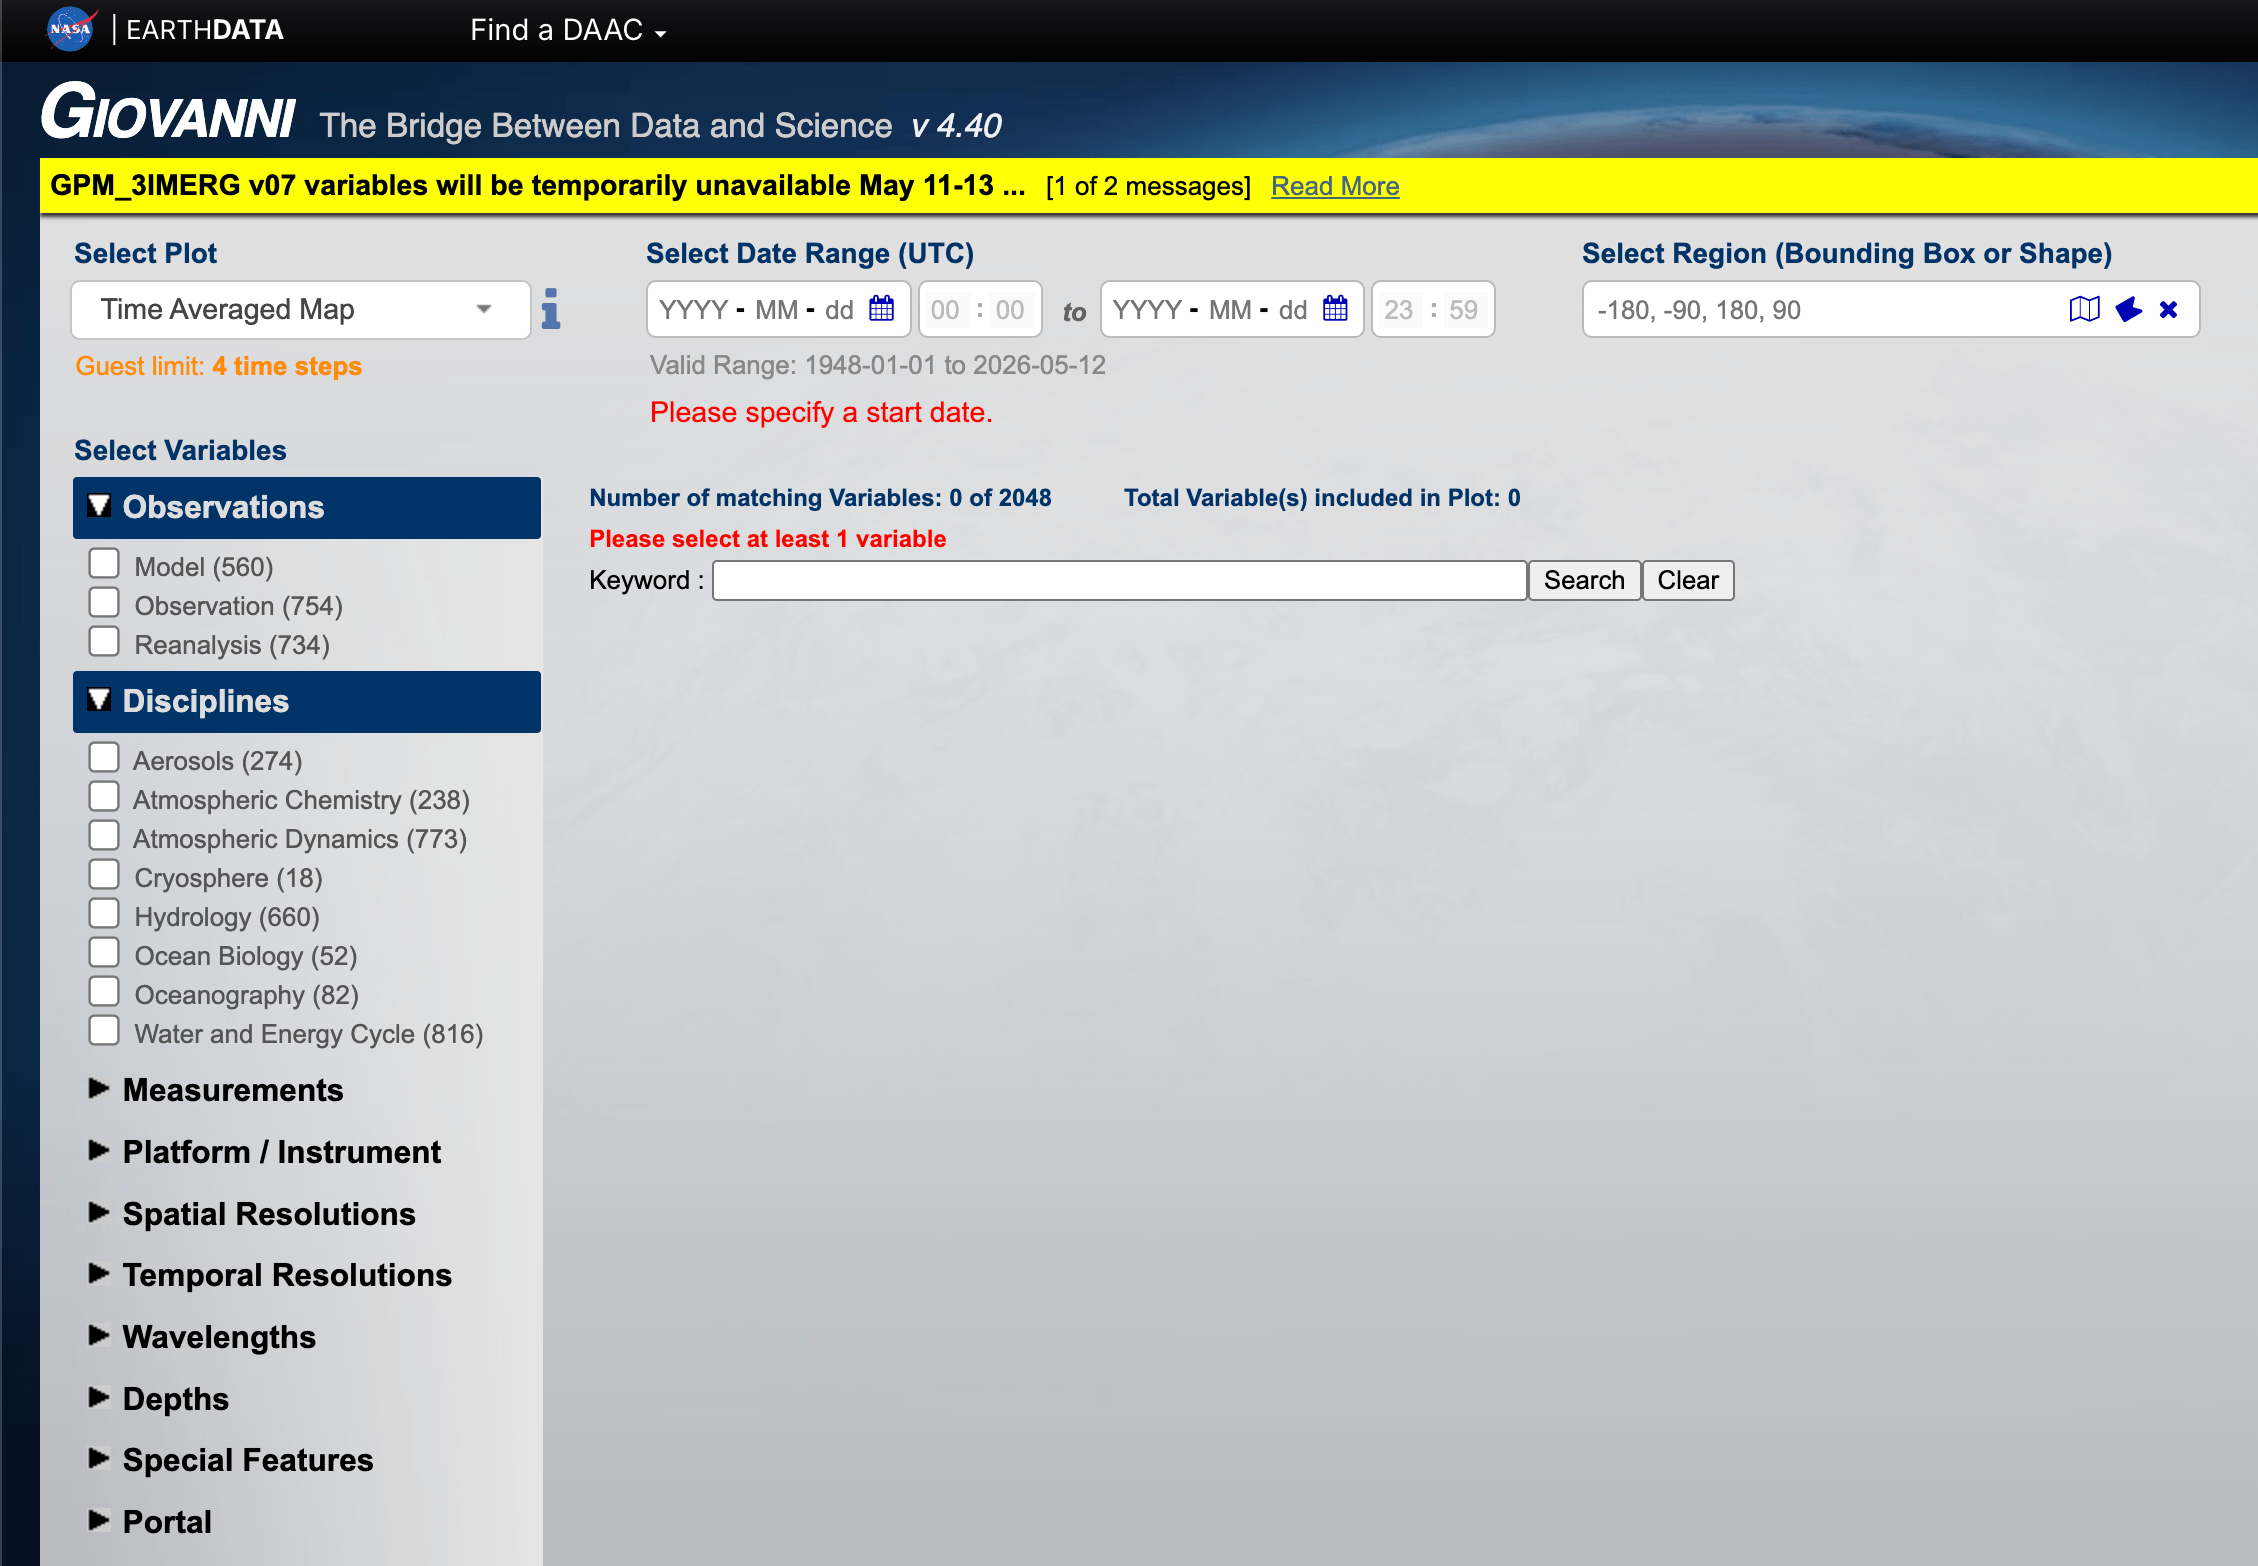
\includegraphics[width=0.9\textwidth]{Images/giovanni.png}
  \caption{NASA Giovanni main interface. Before any data can be retrieved, the
    user must select a plot type, specify a date range, a bounding box, and
    choose from a catalogue of 2{,}048 variables grouped by discipline. The
    empty results panel illustrates why the platform is inaccessible to
  non-specialist users.}
  \label{fig:screenshot_giovanni}
\end{figure}

\subsection{Copernicus Climate Change Service}\label{REL_APPS_COPERNICUS}

The Copernicus Climate Change Service (C3S)~\cite{copernicus}, operated by the
ECMWF on behalf of the European Commission, is the most comprehensive open climate 
data infrastructure currently available. Its Climate Data Store (CDS) provides 
access to terabytes of reanalysis data (ERA5), seasonal forecasts, climate projections, 
and sectoral climate indicators, all under an open licence.

The CDS toolbox allows users to write Python scripts that retrieve, process, and
visualise data from the store, and a graphical interface is provided for simpler
operations. For users willing to engage with the toolbox, the analytical
possibilities are essentially unlimited: custom time periods, arbitrary spatial
domains, user-defined aggregations, and integration with third-party Python
libraries.

Despite this power, the C3S platform shares with NASA Giovanni the fundamental
limitation that it is designed for expert users. Accessing ERA5 data requires
registration, understanding the CDS API, and familiarity with NetCDF file
formats and Python data science libraries. The graphical interface, while
improving, remains complex and slow for simple queries such as ``what is the
typical July temperature in Seville?''. Furthermore, C3S data are reanalysis
products derived from a combination of observations and numerical
weather models,
not the station-interpolated surfaces of WorldClim, so they are suited to
different use cases.

Figure~\ref{fig:screenshot_copernicus} shows the Copernicus Climate Data Store landing page.
\begin{figure}[t]
  \centering
  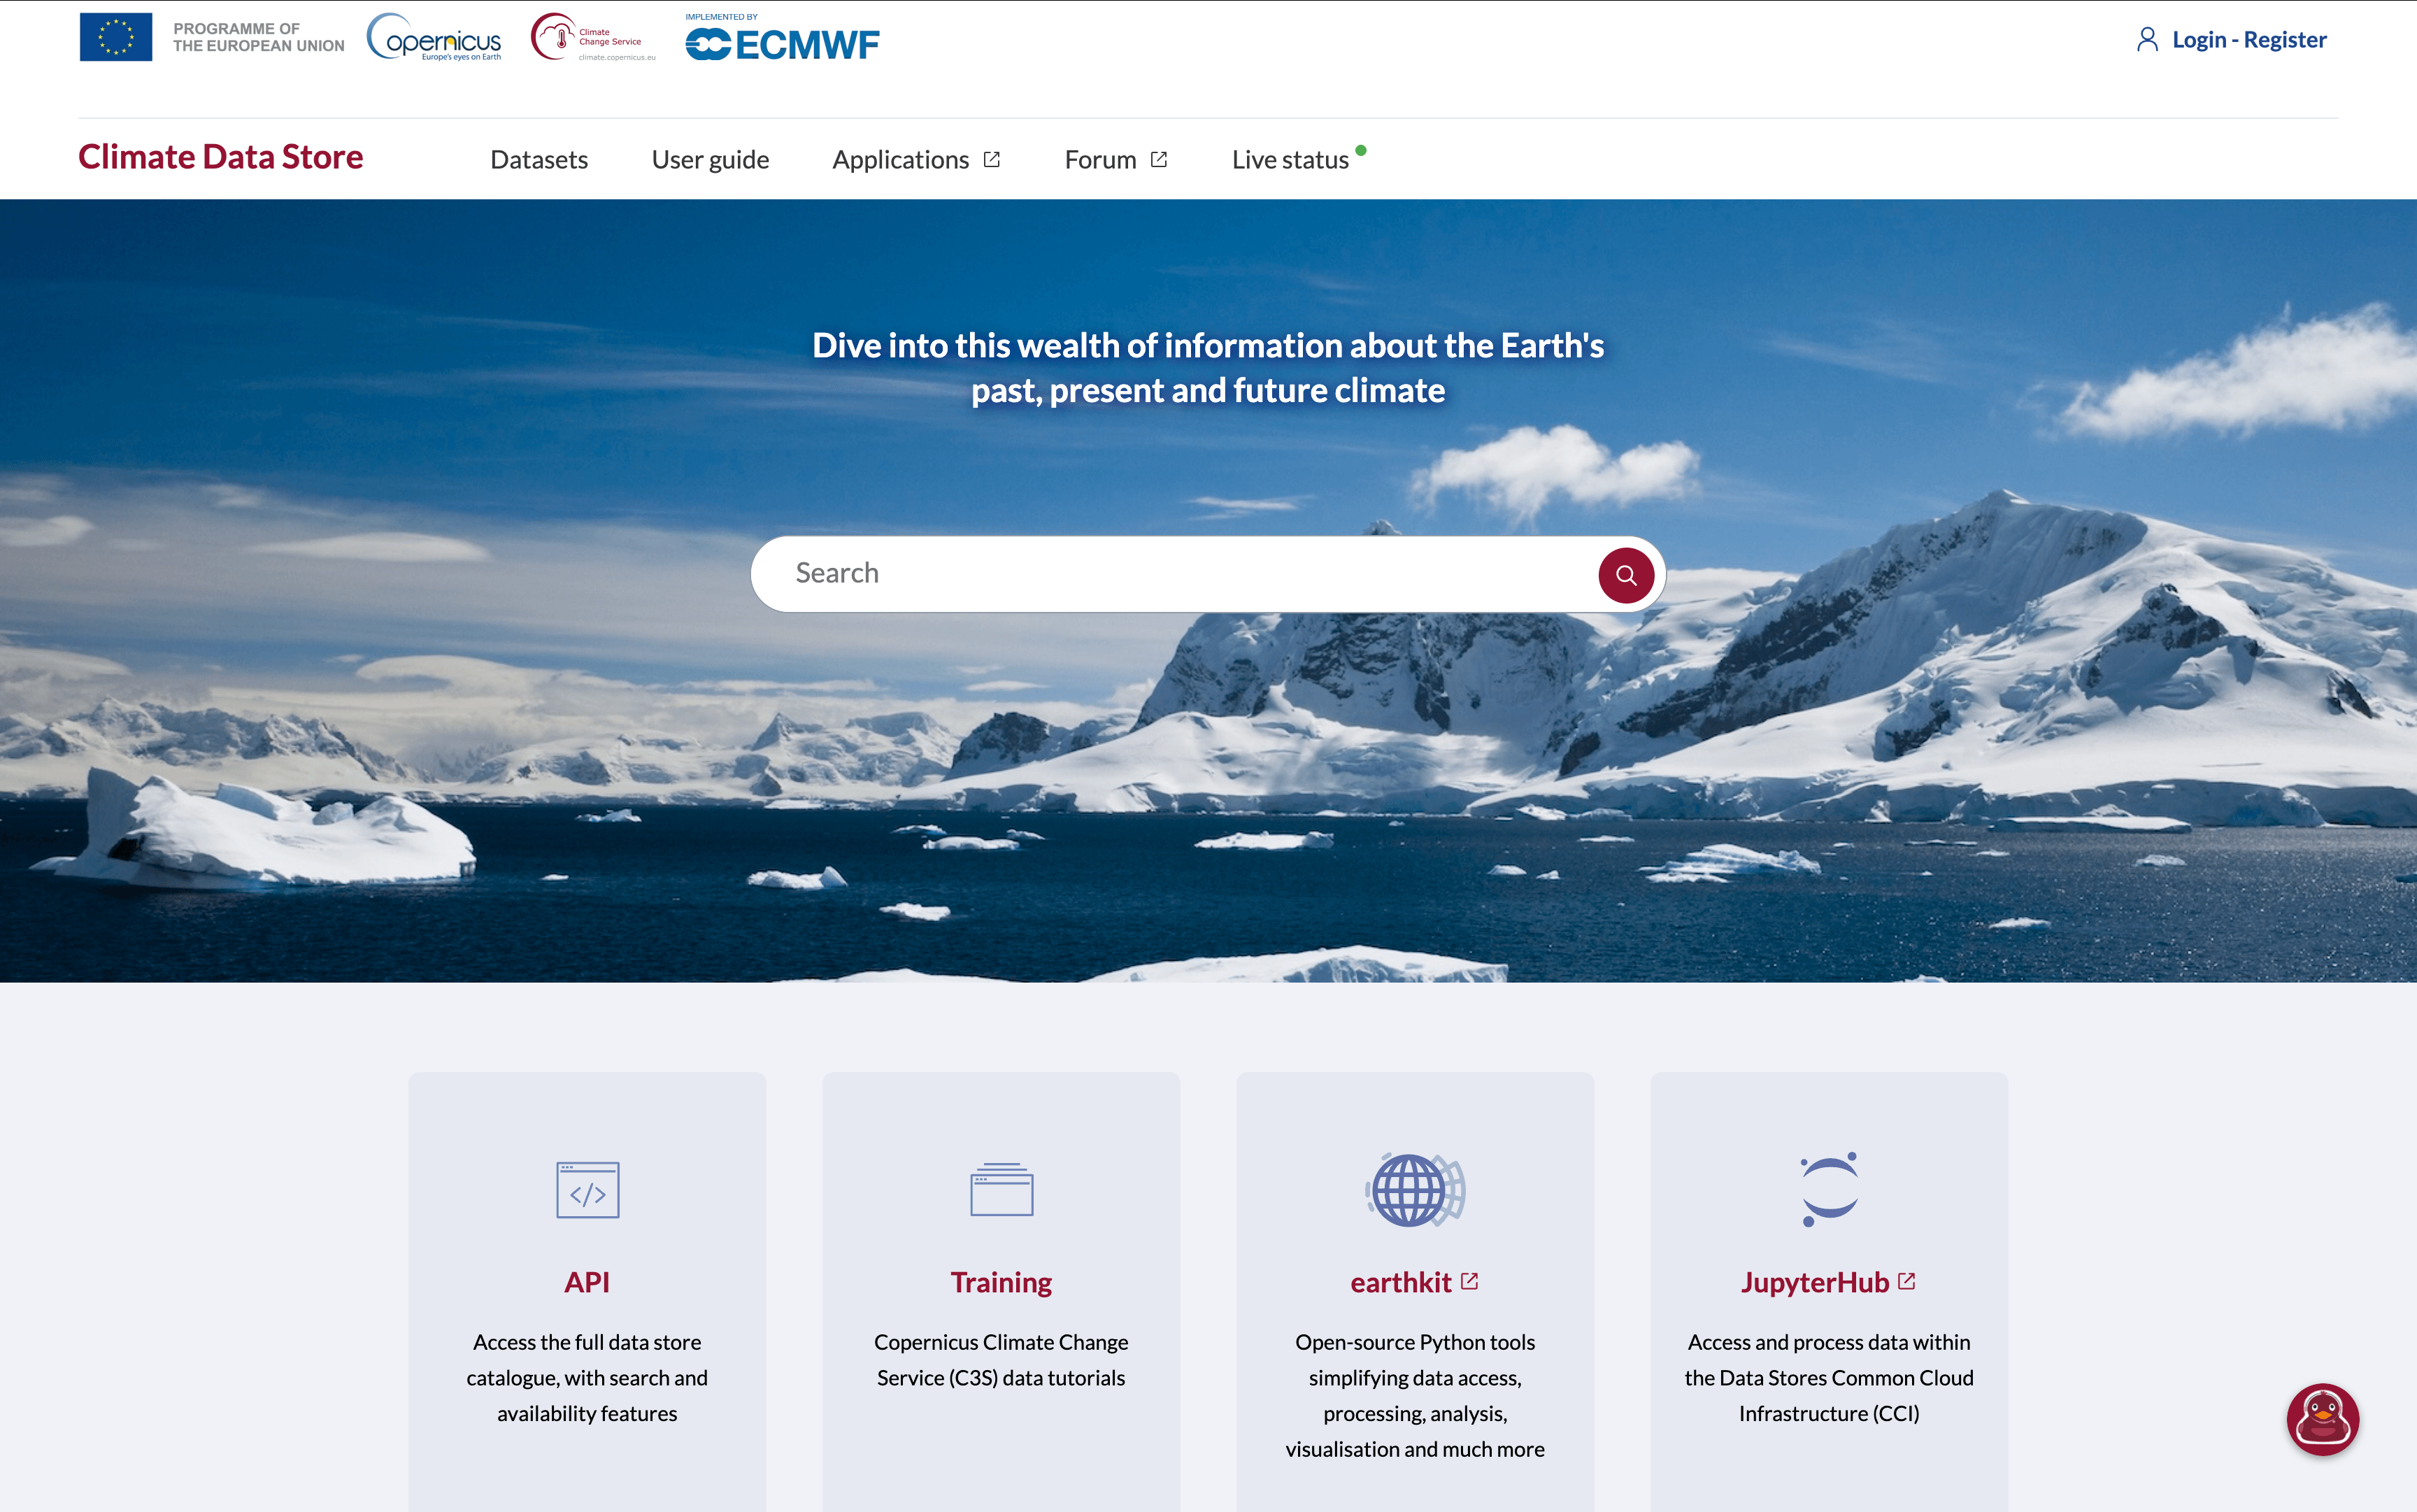
\includegraphics[width=0.9\textwidth]{Images/copernicus.png}
  \caption{Copernicus Climate Data Store landing page. The search-first
    interface and the \emph{Login~/ Register} button in the top-right corner
    illustrate that meaningful access requires both registration and prior
  knowledge of what datasets are available.}
  \label{fig:screenshot_copernicus}
\end{figure}

\subsection{Summary and Opportunity Gap for Climatica}\label{REL_APPS_SUMMARY}

Table~\ref{tab:tools} summarises the capabilities of the tools reviewed above
alongside Climatica. The comparison highlights that no existing tool combines
all of the following in a single, registration-free browser interface: open
kilometre-scale raster data, a Walter-Lieth climatogram, multi-city comparison,
period-based trend exploration, and a regional spatial heatmap.

The two most powerful platforms --- NASA Giovanni and Copernicus C3S --- offer
far greater scientific depth than Climatica, but at the cost of a steep learning
curve that excludes non-specialist users. The simpler tools ---
Climate-Charts.net
and Climate-Data.org --- are accessible but static, offering a single view with
no comparative or temporal dimension. Meteoblue occupies a middle ground but
relies on proprietary data and targets professional users. Climatica would be 
the only tool in this survey that combines ease of use with interactive multi-view
exploration of open, globally consistent raster data.

Figures~\ref{fig:screenshot_climatica_a} and~\ref{fig:screenshot_climatica_b}
show the City Climate page of Climatica for Valladolid, illustrating the map
view, standard climograph, and Walter-Lieth climatogram.
\begin{figure}[t]
  \centering
  \subfigure[Map view with location pin, raster cell outline, and summary stat
  cards.]{
    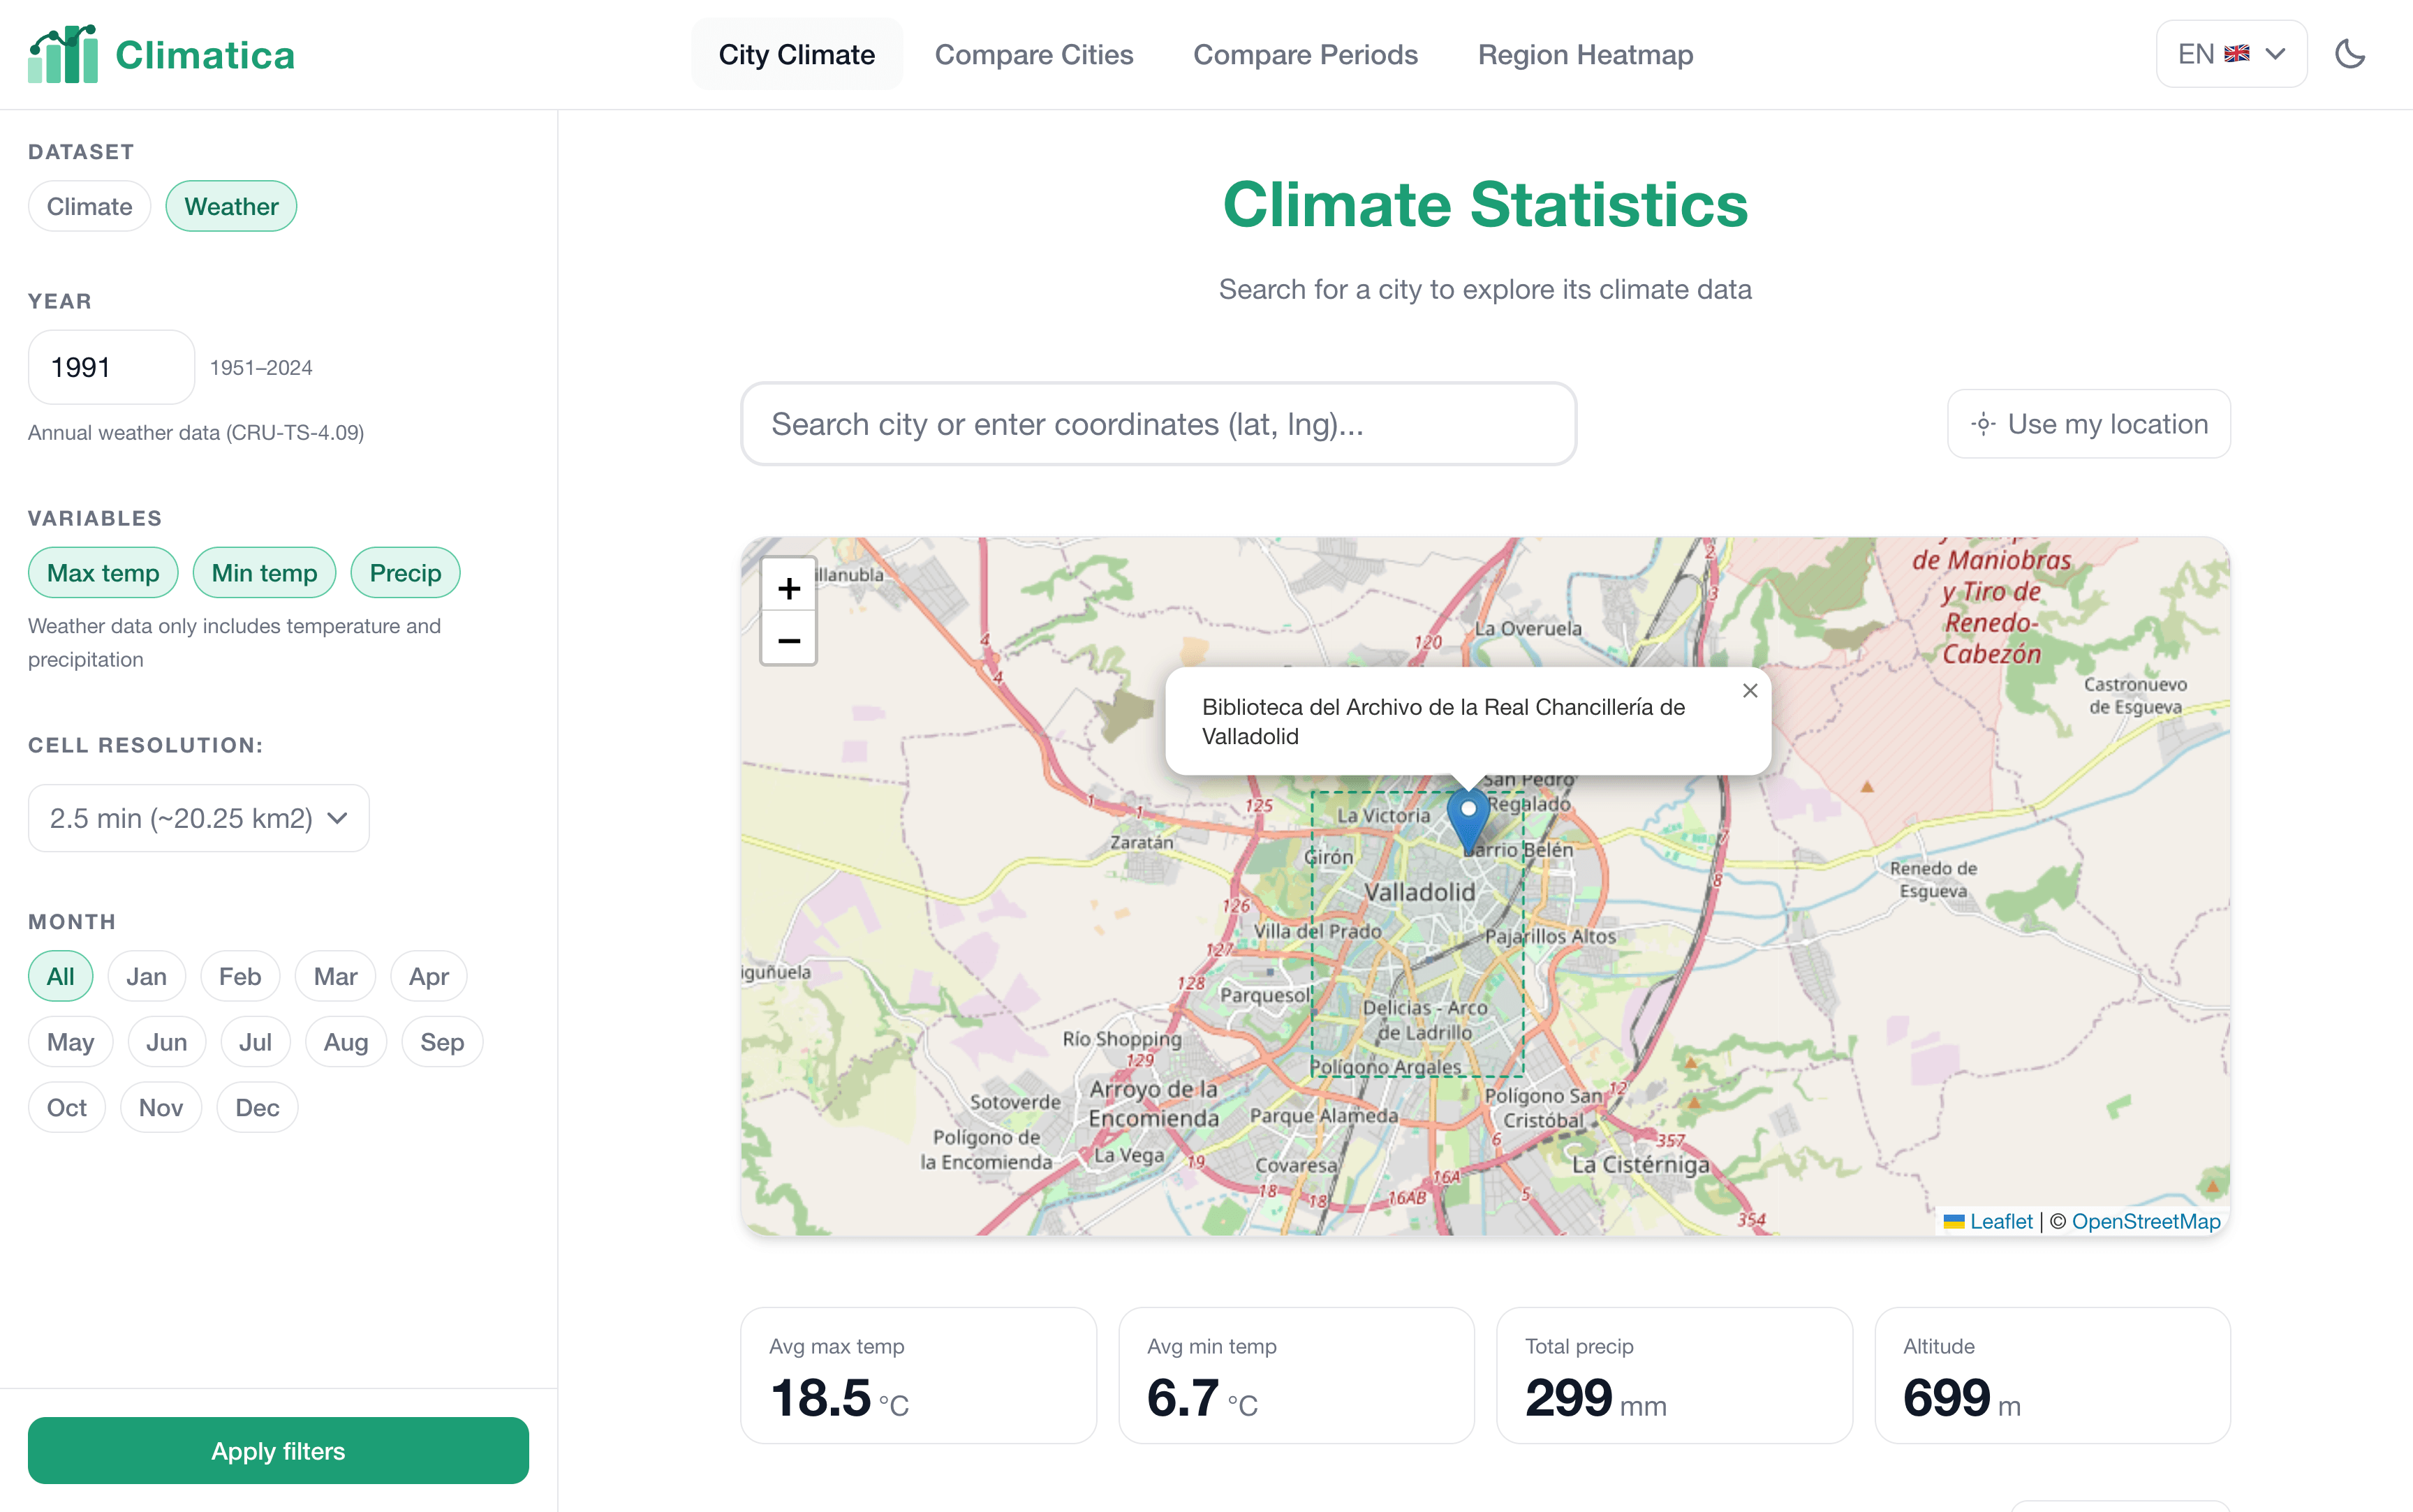
\includegraphics[width=0.9\textwidth]{Images/climatica-map.png}
  }
  \subfigure[Standard climograph: precipitation bars (blue/yellow) and
  temperature lines for the selected city.]{
    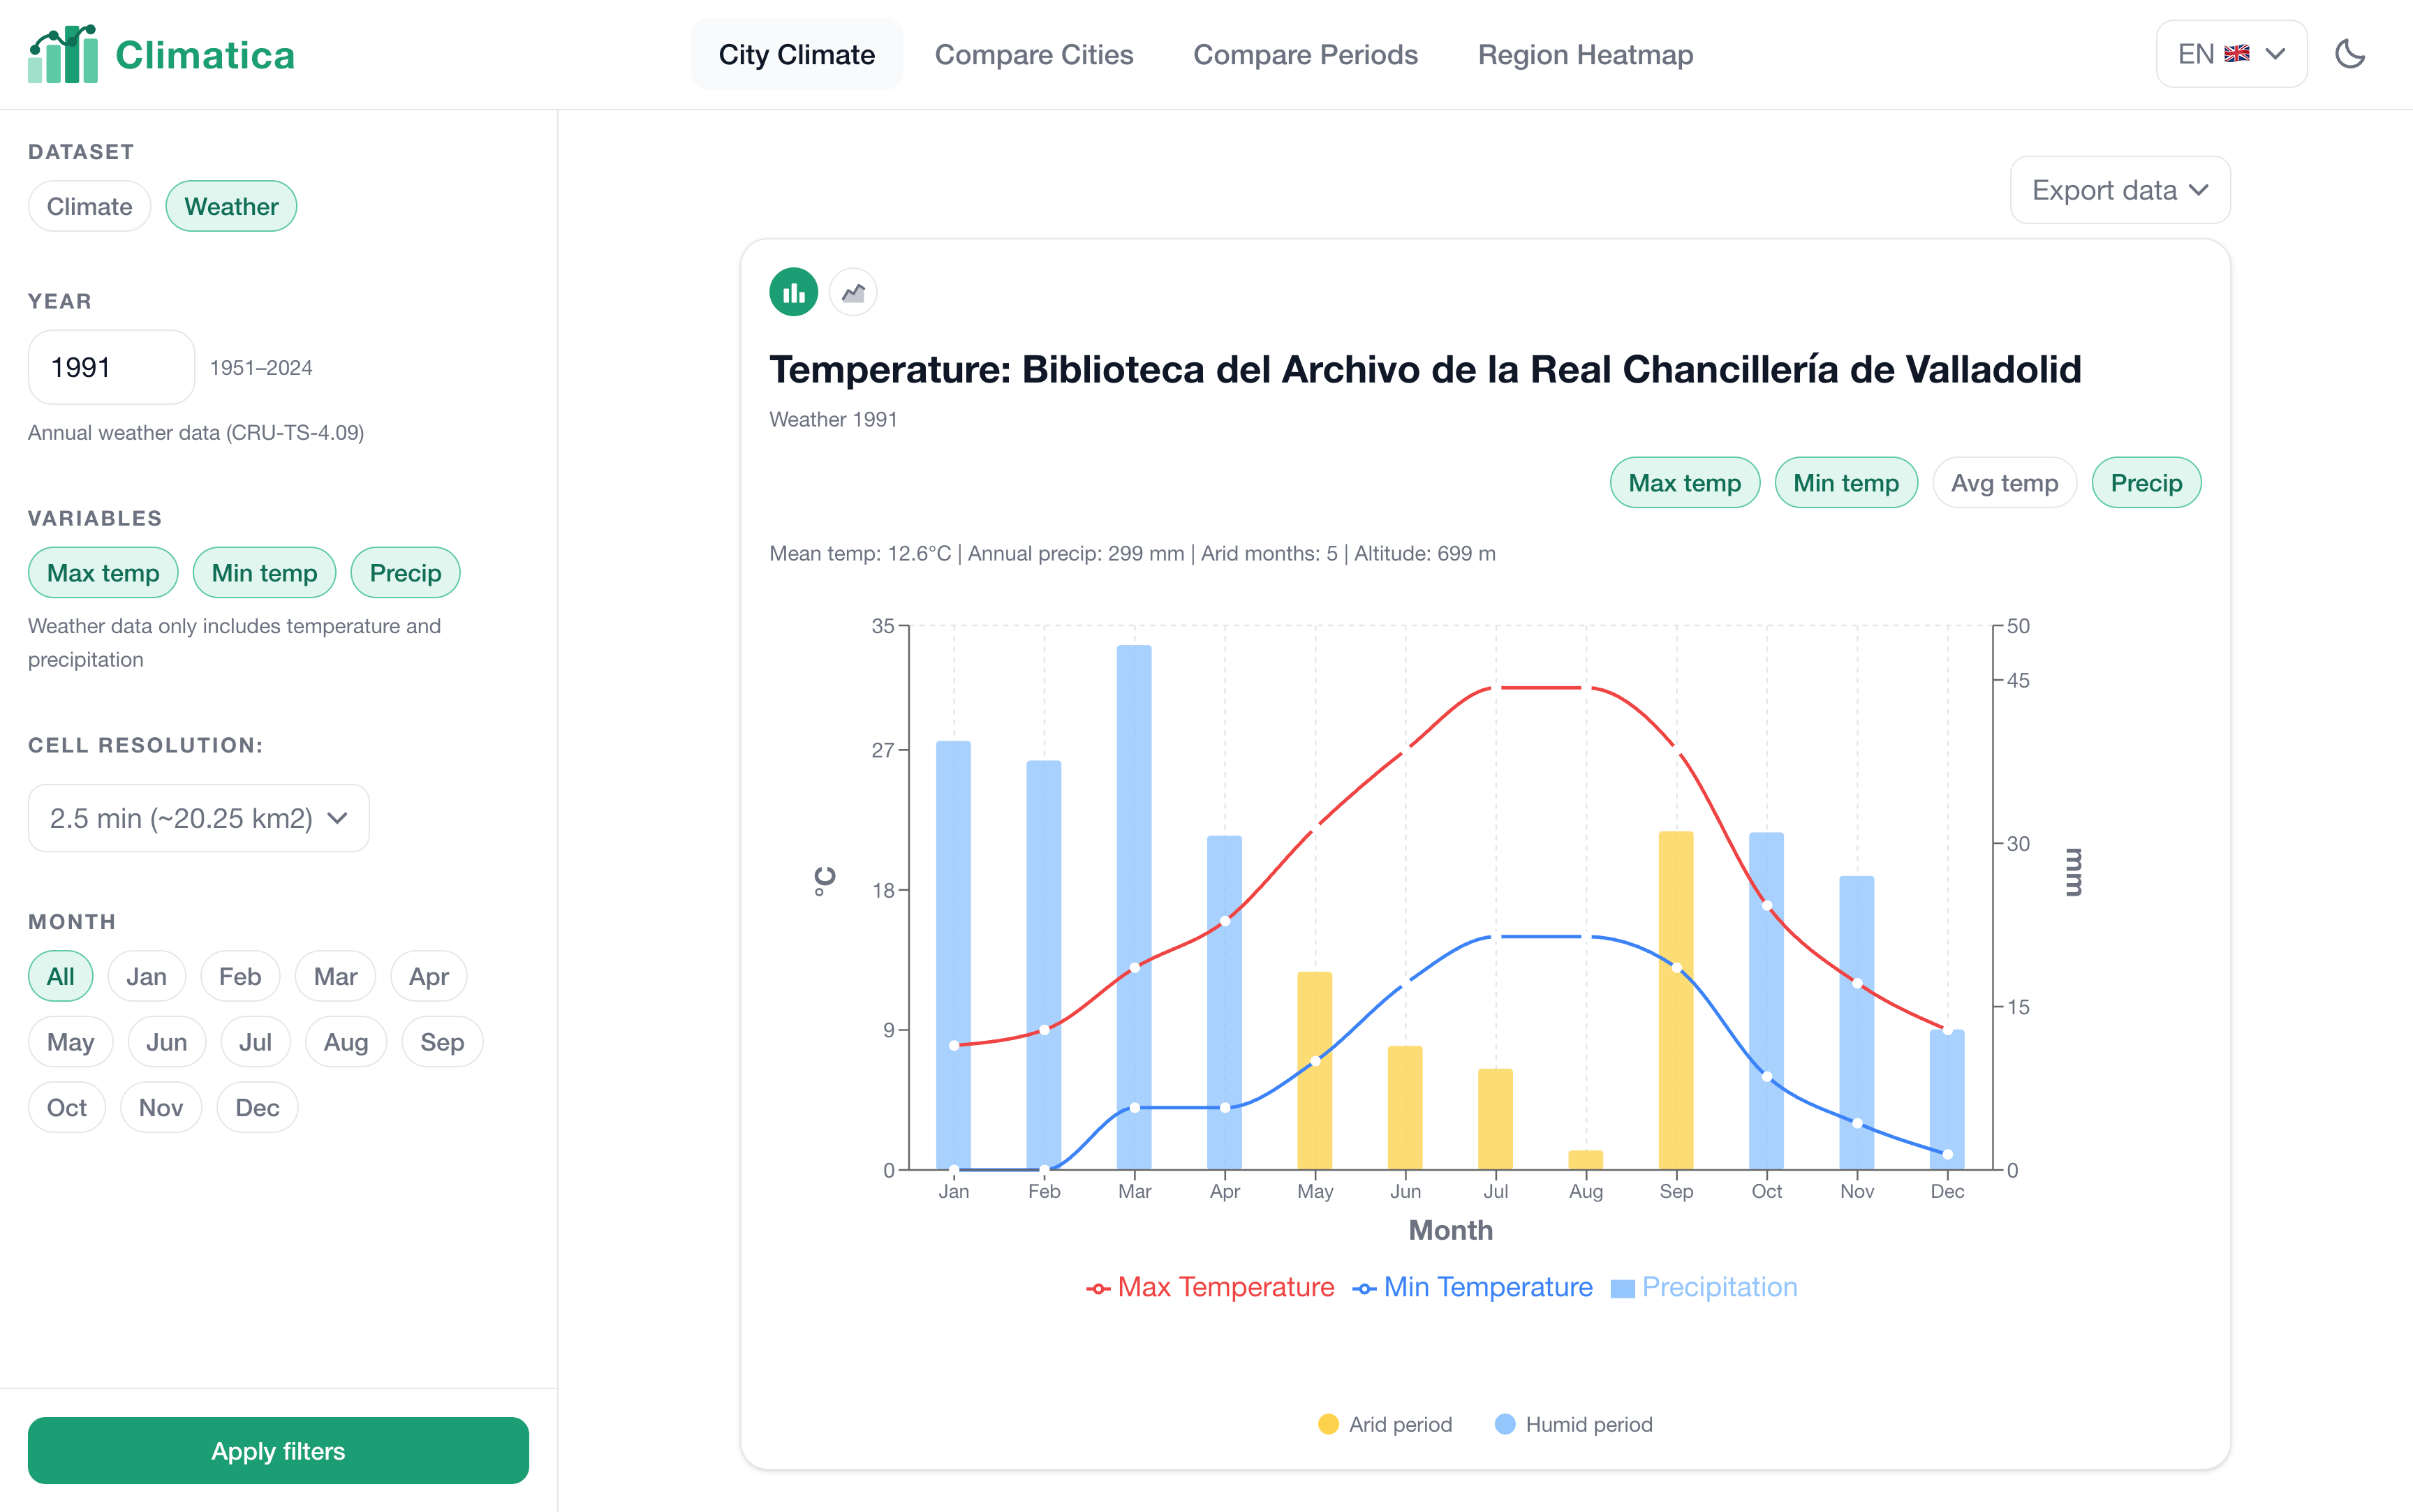
\includegraphics[width=0.9\textwidth]{Images/climatica-columns-graph.png}
  }
  \caption{Climatica City Climate page for Valladolid (weather dataset, year
  1991) --- map and standard climograph views.}
  \label{fig:screenshot_climatica_a}
\end{figure}

\begin{figure}[t]
  \centering
  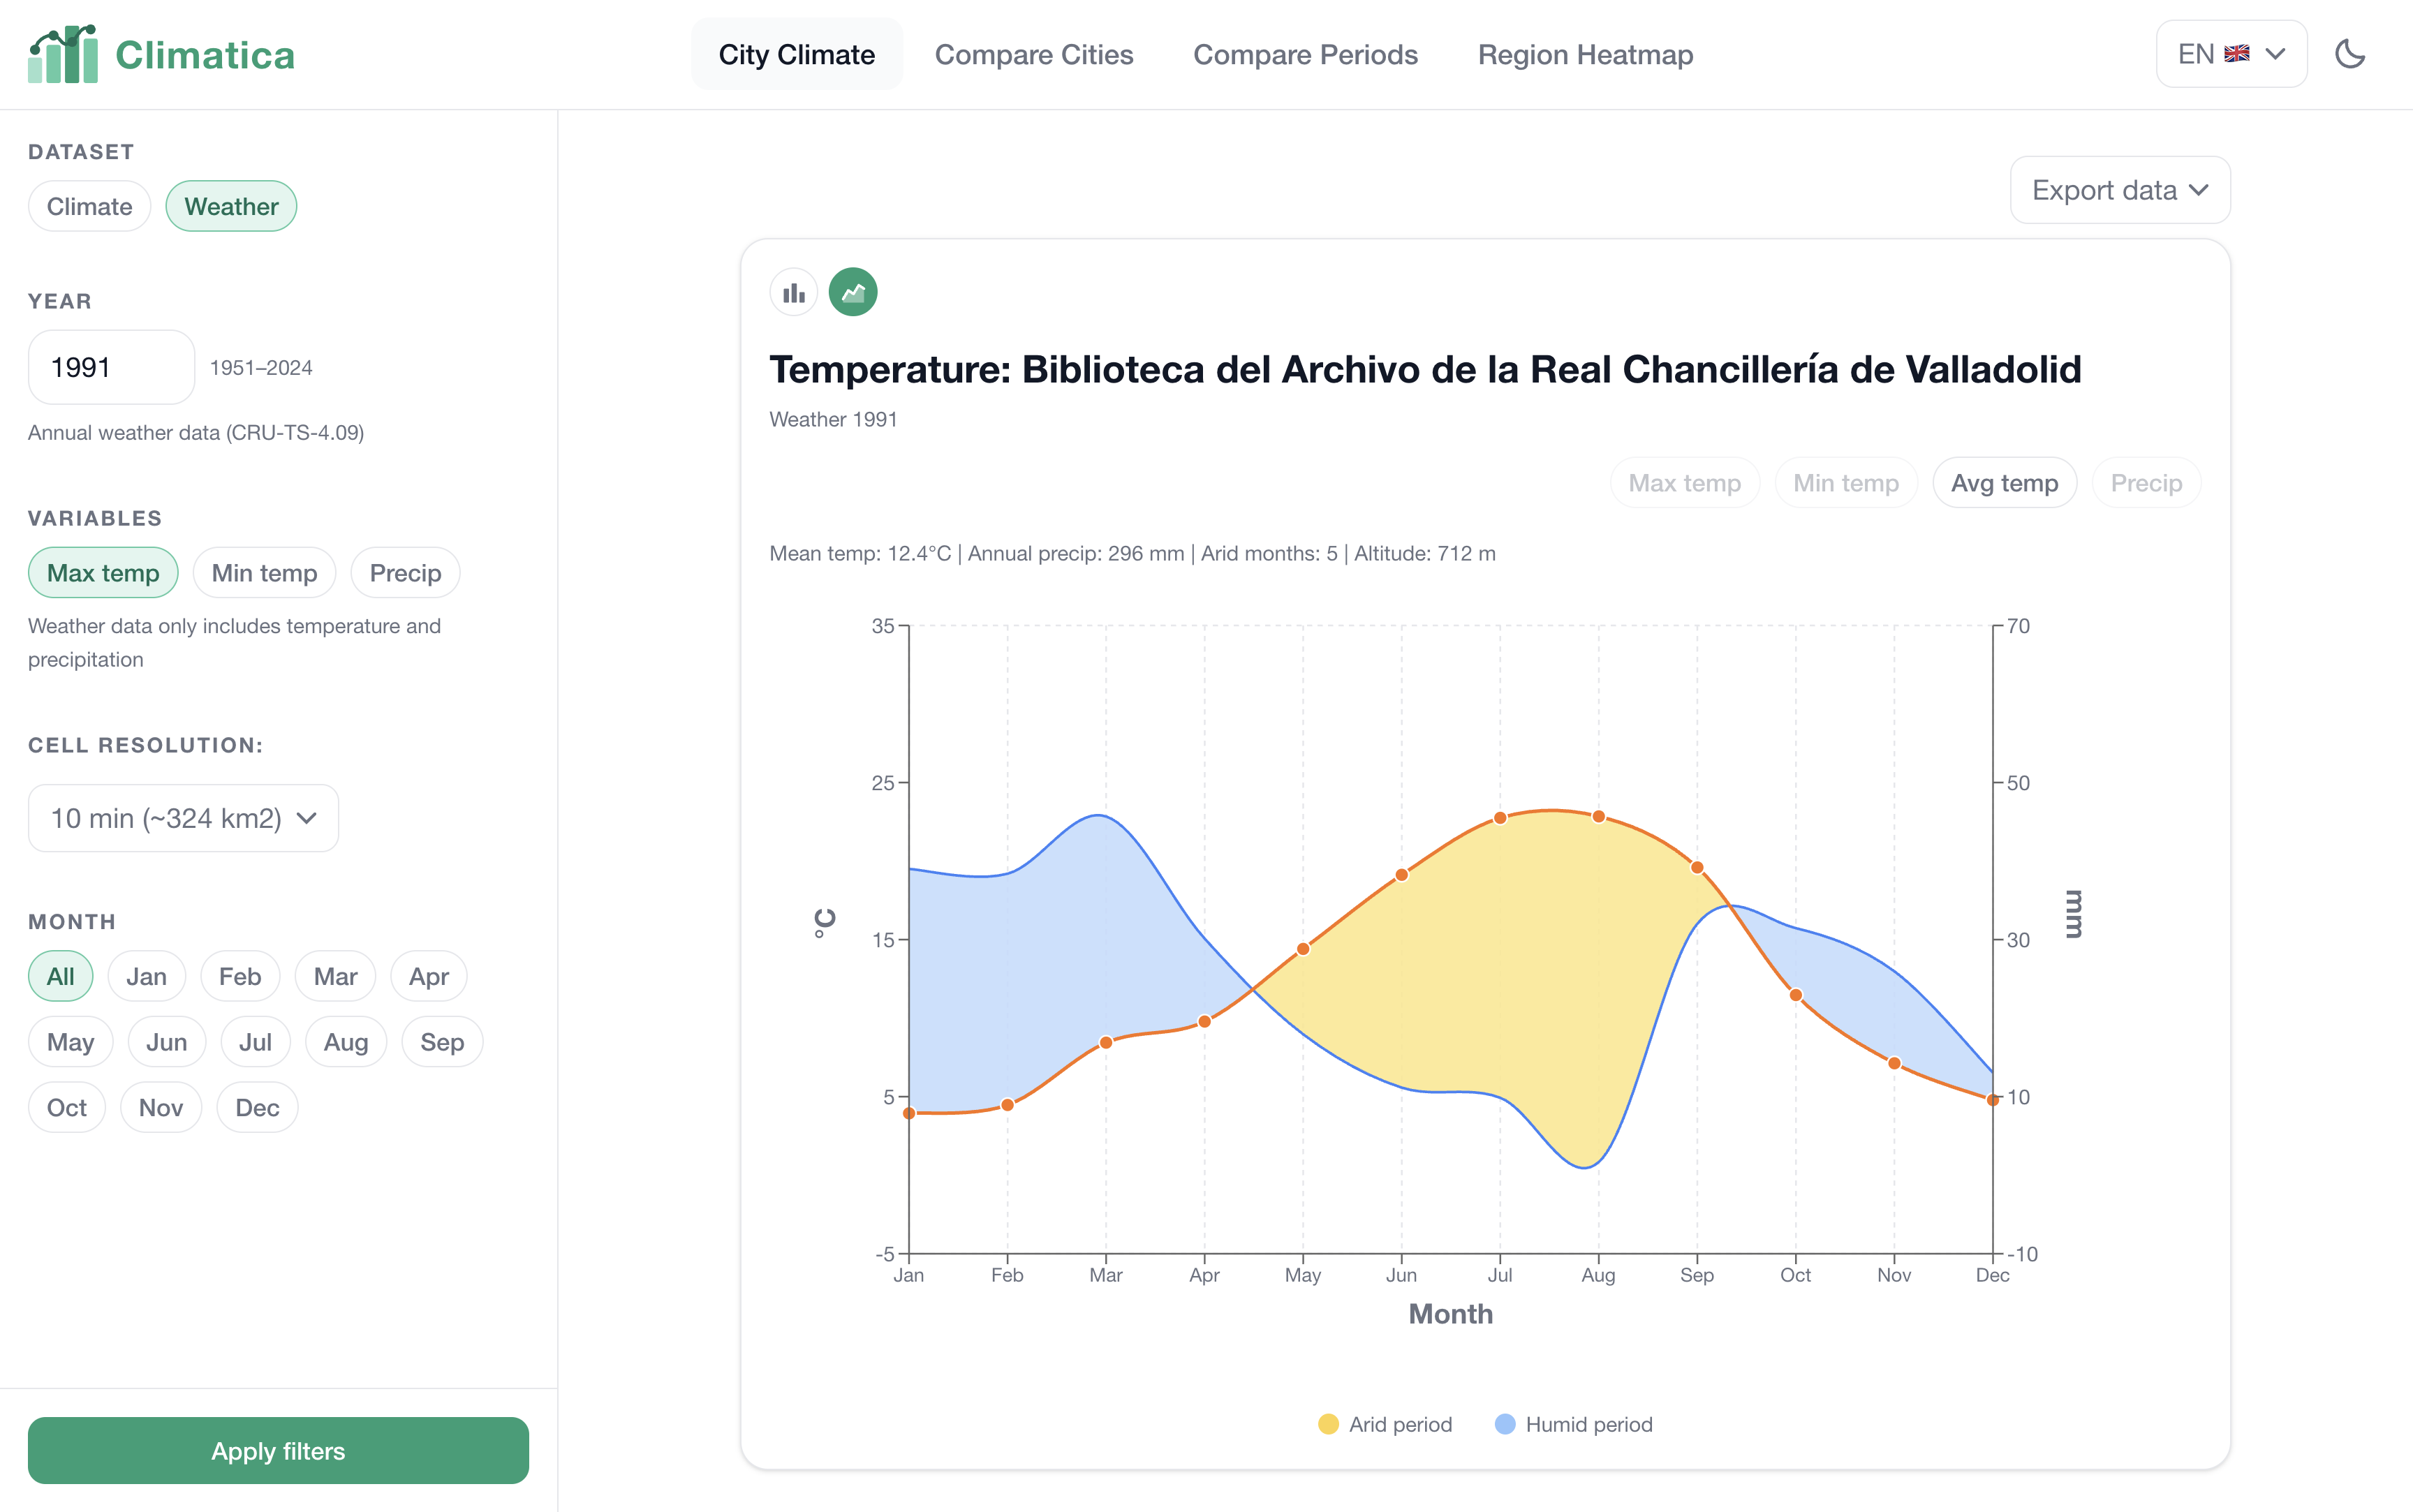
\includegraphics[width=0.9\textwidth]{Images/climatica-walter-lieth.png}
  \caption{Climatica City Climate page --- Walter-Lieth climatogram for the
    same city and period. Yellow areas indicate arid months (summer); blue areas
    indicate humid months (winter and spring). The chart uses SVG
    \texttt{clipPath} with the even-odd winding rule to produce exact arid/humid
  fills without computing curve intersection points explicitly.}
  \label{fig:screenshot_climatica_b}
\end{figure}

\begin{table}[H]
  \centering
  \caption{Comparison of climate data tools.
  \cmark~=~supported, \pmark~=~partial, \xmark~=~not supported.}
  \label{tab:tools}
  \small
  \begin{tabular}{lcccccc}
    \toprule
    \textbf{Feature} &
    \textbf{\shortstack{Climate\\Charts}} &
    \textbf{\shortstack{Climate\\Data.org}} &
    \textbf{Meteoblue} &
    \textbf{\shortstack{NASA\\Giovanni}} &
    \textbf{\shortstack{Copernicus\\C3S}} &
    \textbf{Climatica} \\
    \midrule
    City climate profile      & \cmark & \cmark & \cmark  & \xmark &
    \xmark & \cmark \\
    Walter-Lieth climatogram  & \cmark & \cmark & \xmark  & \xmark &
    \xmark & \cmark \\
    Multi-city comparison     & \xmark & \xmark & \pmark  & \xmark &
    \xmark & \cmark \\
    Period trend comparison   & \xmark & \xmark & \pmark  & \cmark &
    \cmark & \cmark \\
    Regional spatial heatmap  & \xmark & \xmark & \xmark  & \cmark &
    \cmark & \cmark \\
    Open km-scale data        & \xmark & \xmark & \xmark  & \cmark &
    \cmark & \cmark \\
    No registration required  & \cmark & \cmark & \pmark  & \xmark &
    \xmark & \cmark \\
    Non-specialist audience   & \cmark & \cmark & \xmark  & \xmark &
    \xmark & \cmark \\
    \bottomrule
  \end{tabular}
  \normalsize
\end{table}

% * ─── 2.2 WorldClim ────────────────────────────────────────────────────────────

\section{WorldClim}\label{REL_WORLDCLIM}

\subsection{The Dataset}\label{REL_WORLDCLIM_DATA}

WorldClim is a global database of high-resolution climate data widely used in
ecology, biogeography, agriculture, and climate-change research. Version~2.1,
described by Fick and Hijmans~\cite{fick2017worldclim}, provides interpolated
monthly climate surfaces derived from weather-station observations collected
between 1970 and 2000. The dataset covers the entire land surface of the Earth
at four spatial resolutions: 10 arc-minutes ($\approx$18.5\,km at the equator),
5 arc-minutes ($\approx$9.2\,km), 2.5 arc-minutes ($\approx$4.6\,km), and 30
arc-seconds ($\approx$900\,m).

Seven monthly variables are available in the climate dataset: minimum
temperature
(\texttt{tmin}), maximum temperature (\texttt{tmax}), average temperature
(\texttt{tavg}), precipitation (\texttt{prec}), solar radiation (\texttt{srad}),
wind speed (\texttt{wind}), and vapour pressure (\texttt{vapr}). Climatica uses
\texttt{tmin}, \texttt{tmax}, \texttt{tavg}, and \texttt{prec} --- the four
variables most relevant to general climate characterisation and to the
construction of Walter-Lieth climatograms.

\subsubsection{Bioclimatic Variables}\label{REL_WORLDCLIM_BIO}

In addition to the seven monthly variables, WorldClim provides 19 bioclimatic
variables (BIO1--BIO19) derived algorithmically from the monthly temperature and
precipitation series. These variables were designed to capture biologically
meaningful aspects of climate that are not immediately apparent from the raw
monthly values, and they are widely used as predictors in species distribution
models and ecological niche analyses.

Table~\ref{tab:bio} lists the 19 bioclimatic variables. Several of them have
intuitive interpretations: BIO1 is simply the annual mean temperature, BIO12 is
the total annual precipitation, and BIO4 (temperature seasonality) measures how
much monthly temperatures vary across the year. Others capture more specific
relationships, such as BIO8 (mean temperature of the wettest quarter) and BIO18
(precipitation of the warmest quarter), which are particularly relevant for
understanding vegetation patterns in seasonally dry regions.

\begin{table}[H]
  \centering
  \caption{WorldClim bioclimatic variables (BIO1--BIO19).}
  \label{tab:bio}
  \begin{tabular}{ll}
    \toprule
    \textbf{Code} & \textbf{Description} \\
    \midrule
    BIO1  & Annual Mean Temperature \\
    BIO2  & Mean Diurnal Range (Mean of monthly max$-$min) \\
    BIO3  & Isothermality (BIO2/BIO7 $\times$ 100) \\
    BIO4  & Temperature Seasonality (standard deviation $\times$ 100) \\
    BIO5  & Max Temperature of Warmest Month \\
    BIO6  & Min Temperature of Coldest Month \\
    BIO7  & Temperature Annual Range (BIO5$-$BIO6) \\
    BIO8  & Mean Temperature of Wettest Quarter \\
    BIO9  & Mean Temperature of Driest Quarter \\
    BIO10 & Mean Temperature of Warmest Quarter \\
    BIO11 & Mean Temperature of Coldest Quarter \\
    BIO12 & Annual Precipitation \\
    BIO13 & Precipitation of Wettest Month \\
    BIO14 & Precipitation of Driest Month \\
    BIO15 & Precipitation Seasonality (Coefficient of Variation) \\
    BIO16 & Precipitation of Wettest Quarter \\
    BIO17 & Precipitation of Driest Quarter \\
    BIO18 & Precipitation of Warmest Quarter \\
    BIO19 & Precipitation of Coldest Quarter \\
    \bottomrule
  \end{tabular}
\end{table}

Although Climatica does not currently expose the bioclimatic variables in its
user interface --- focusing instead on the monthly temperature and precipitation
series that are more interpretable for general users --- the SCRAPI API provides
full access to them, and they represent a natural direction for future extension
of the application.

\subsubsection{Interpolation Methodology}\label{REL_WORLDCLIM_INTERP}

The WorldClim surfaces are not direct observations: they are the result of a
spatial interpolation procedure applied to records from tens of thousands of
weather stations distributed unevenly across the globe. The interpolation method
used in WorldClim~2.1 is ANUSPLIN~\cite{hutchinson1995}, a thin-plate smoothing
spline algorithm that models the relationship between a climate variable and
geographic predictors --- primarily latitude, longitude, and elevation.

Elevation plays a particularly important role because temperature decreases with
altitude at a relatively predictable rate (the environmental lapse rate), while
orographic effects strongly influence precipitation on windward and leeward
slopes. By incorporating a digital elevation model as a covariate, ANUSPLIN can
produce surfaces that reflect the local topographic influence on climate even in
areas with sparse station coverage.

The quality of the interpolation varies across the globe. In densely observed
regions such as Europe and North America, the surfaces are highly reliable, with
root-mean-square errors of less than 0.5\,$^\circ$C for temperature. In
data-sparse regions such as the Sahara, central Asia, and the Amazon basin,
uncertainty is higher. This limitation is inherent to any station-based
interpolation product and is shared by all tools that use WorldClim as their
data source, including Climatica.

\subsubsection{Historical Weather Data and Climate
Normals}\label{REL_WORLDCLIM_PERIODS}

Alongside the baseline climate data, WorldClim also distributes historical
monthly weather data for the period 1951--2024, prepared from the CRU-TS-4.09
dataset~\cite{harris2020cru}. CRU-TS (Climatic Research Unit gridded Time
Series) is produced by the University of East Anglia and provides monthly
gridded fields of temperature and precipitation derived from station
observations, covering the global land surface since 1901.

From the CRU-TS-based weather rasters, WorldClim has computed additional 30-year
climate normals for the periods 1951--1980, 1961--1990, 1981--2010, and
1991--2020. Together with the original 1970--2000 baseline, this gives five
overlapping 30-year periods that can be compared to detect long-term trends.
Climatica exposes all five periods in its Period Comparison page, allowing a
user to see, for example, whether summer temperatures in a particular city have
risen consistently across successive 30-year averages.

The raw data are distributed as GeoTIFF raster files. The complete archive
consists of 8{,}836 files totalling approximately 85.6\,GB. Converted naively
to RDF triples for a semantic triplestore, the archive would yield roughly
375 billion triples requiring 17.7\,petabytes of storage --- approximately
332 times the capacity of a typical Virtuoso deployment configured with
16\,GB of RAM~\cite{scrapi}. Even the grid metadata alone, before any pixel
values are considered, amounts to over 16 billion triples across the four
spatial resolutions. Working with the raw files directly requires GIS software
or programming libraries such as GDAL or rasterio --- and this scale is
precisely the motivation for the virtual graph approach adopted by SCRAPI
(Section~\ref{REL_WORLDCLIM_API}).

\subsection{The Virtual Semantic API}\label{REL_WORLDCLIM_API}

To make WorldClim data accessible over the web without requiring GIS expertise,
Guillermo Vega Gorgojo at the Universidad de Valladolid developed the WorldClim
Virtual Semantic API~\cite{scrapi}, hereafter referred to as SCRAPI. The design
of SCRAPI is motivated by a scalability problem inherent in the materialisation
approach to semantic spatial data.

A straightforward way to expose raster data as Linked Data would be to convert
every pixel into RDF triples and load them into a SPARQL triplestore. For the
complete WorldClim archive this would produce approximately 375 billion triples,
requiring around 17.7\,petabytes of storage --- far beyond what a typical
Virtuoso deployment can handle. A W3C Working Group Note on spatial data on the
web explicitly discourages full materialisation of large raster datasets for
this reason~\cite{w3c_spatial}.

SCRAPI instead adopts a \emph{virtual graph} approach: no RDF is materialised
in advance. Queries are answered at request time by the GDAL library reading
directly from the GeoTIFF files, while the API surface is identical to what a
fully materialised triplestore would expose. The result is a lightweight, fast,
and scalable REST service that answers climatic and weather queries at any
available resolution for any location on Earth.

\subsubsection{Data Model}\label{REL_WORLDCLIM_API_MODEL}

SCRAPI organises WorldClim data into four hierarchical resource types, each
identified by an IRI:

\begin{itemize}
  \item \textbf{Grid.} A spatial resolution level. Four grids are defined:
    \texttt{Grid\_10m}, \texttt{Grid\_5m}, \texttt{Grid\_2.5m}, and
    \texttt{Grid\_30s}. Each grid is described by its number of rows and
    columns, its cell dimensions in degrees, and the full list of raster IRIs
    it contains.

  \item \textbf{Cell.} A single rectangular tile within a grid. A cell is
    identified by its row and column indices (e.g.\
    \texttt{Cell\_30s\_r5758c21057}). Its representation includes a polygon in
    WKT format, a centroid, an elevation value, and the IRIs of all pixels
    located within it.

  \item \textbf{Raster.} A monthly or yearly dataset for one variable and one
    time period (e.g.\ \texttt{Raster\_2.5m\_tmax\_w1996}). Because each
    GeoTIFF file contains a single band, twelve files correspond to a single
    monthly raster in the API model; SCRAPI models them as one raster with
    twelve bands. This reduces the total number of raster objects from 8,836
    files to 806 logical rasters.

  \item \textbf{Pixel.} The intersection of a cell and a raster --- the
    fundamental unit of climate data. A pixel IRI encodes the grid resolution,
    the cell coordinates, the variable, and the time period (e.g.\
    \texttt{Pixel\_2.5m\_r1151c4211\_prec\_w1953}). Its representation returns
    one numerical value per month (\texttt{valueMonth01} through
    \texttt{valueMonth12}), with temperatures in tenths of a degree Celsius and
    precipitation in millimetres.
\end{itemize}

\subsubsection{API Operations}\label{REL_WORLDCLIM_API_OPS}

The API exposes four generic operations, all authenticated with a Bearer token:

\begin{itemize}
  \item \texttt{GET /resource?id=\{type\}\&iri=\{iri\}} --- retrieve the
    representation of a single resource.
  \item \texttt{GET /resources?id=\{type\}\&iris=\{iri\}...} --- retrieve
    multiple resources in one request, reducing round-trips.
  \item \texttt{GET /query?id=\{queryId\}\&\{params\}} --- execute a named
    parametrised query.
\end{itemize}

Named queries cover the most common access patterns. The \texttt{cellofpoint}
query returns the cell that contains a given latitude/longitude pair for each
available grid resolution. \texttt{pixelsofapoint} returns all pixel IRIs
associated with a point, filterable by grid, variable, time period, and dataset
type (climate or weather). \texttt{pixelvaluesofapoint} extends this by
including the actual monthly values, avoiding a second round-trip to fetch each
pixel individually.

For regional queries, \texttt{cellsinbox} and \texttt{pixelsinbox} accept a
bounding box defined by north, south, east, and west coordinates; the polygon
variants (\texttt{cellsinpolygonGEO}, \texttt{pixelsinpolygonGEO}) accept an
arbitrary WKT polygon. Results are paginated via \texttt{limit} and
\texttt{offset} parameters. The \texttt{avgpixelvaluesinbox} and
\texttt{avgpixelvaluesinpolygonGEO} queries aggregate pixel values into a single
average per raster and month, which is the operation used by Climatica's heatmap
page to summarise data across a user-drawn region.

\subsubsection{Usage in Climatica}\label{REL_WORLDCLIM_API_USAGE}

Climatica calls SCRAPI through server-side route handlers. The typical flow for
the City Climate page is as follows: the application first resolves the selected
city's coordinates to a cell IRI via \texttt{cellofpoint}; it then calls
\texttt{pixelvaluesofapoint} with the desired grid, variable set
(\texttt{tmin}, \texttt{tmax}, \texttt{tavg}, \texttt{prec}), and climate period
to retrieve all twelve monthly values in a single request. The Period Comparison
page issues multiple such requests in parallel and overlays the results. The
Heatmap page uses \texttt{pixelvaluesinbox} or \texttt{pixelsinpolygonGEO} with
the user-drawn selection, parsing pixel IRIs to reconstruct the
geographic bounds
of each tile and colour-coding each cell according to its value.

% * ─── 2.3 Semantic Web and Linked Data ─────────────────────────────────────────
\section{Semantic Web and Linked Data}\label{REL_SEMWEB}

\subsection{The Resource Description Framework}\label{REL_SEMWEB_RDF}

The Semantic Web is a vision, first articulated by
Tim Berners-Lee~\cite{bernerslee2001}, of a web in which data published on the
internet carry enough structure and meaning that machines can process and
integrate them automatically, without human intervention. The foundational data
model underlying this vision is the \emph{Resource Description Framework}
(RDF)~\cite{rdf11}.

RDF represents knowledge as a set of \emph{triples}, each consisting of three
components:

\begin{itemize}
  \item \textbf{Subject} --- the resource being described, identified by an IRI
    (Internationalised Resource Identifier) or a blank node.
  \item \textbf{Predicate} --- the property or relationship, always an IRI.
  \item \textbf{Object} --- the value of the property, either another IRI or a
    literal (a string, number, or date).
\end{itemize}

For example, the fact that Madrid is a city with coordinates $40.4^\circ$\,N,
$3.7^\circ$\,W can be expressed as two triples:
\begin{center}
  \texttt{wd:Q2807} \quad \texttt{wdt:P31} \quad \texttt{wd:Q515} \\
  \texttt{wd:Q2807} \quad \texttt{wdt:P625} \quad \texttt{"40.4 -3.7"}
\end{center}
where \texttt{wd:Q2807} is the IRI for Madrid, \texttt{wdt:P31} means
\emph{instance of}, \texttt{wd:Q515} is the IRI for \emph{city}, and
\texttt{wdt:P625} is the IRI for \emph{coordinate location}.

A collection of RDF triples forms a \emph{graph}: the subjects and objects are
nodes, and the predicates are directed edges. This graph structure makes it
natural to express not just individual facts but also relationships between
facts --- and to traverse chains of relationships that would require complex
joins in a relational database.

\subsection{SPARQL}\label{REL_SEMWEB_SPARQL}

SPARQL (SPARQL Protocol and RDF Query Language)~\cite{sparql11} is the standard
query language for RDF graphs, playing the same role that SQL plays for
relational databases. A SPARQL query describes a \emph{graph pattern}: a set of
triple patterns with variables in place of some IRIs or literals. The query
engine searches the RDF graph for all assignments of values to variables that
make every triple pattern true, and returns the results as a table.

A simple illustrative query against the Wikidata graph might ask for
all entities
that are instances of \emph{human settlement}:

\begin{lstlisting}[language=SPARQL, caption={A basic SPARQL query over Wikidata.},
  label={lst:sparql_basic}]
SELECT ?city ?cityLabel WHERE {
  ?city wdt:P31/wdt:P279* wd:Q486972 .
  SERVICE wikibase:label {
    bd:serviceParam wikibase:language "en" .
  }
}
\end{lstlisting}

The path expression \texttt{wdt:P31/wdt:P279*} means: follow the \emph{instance
of} predicate once, then follow \emph{subclass of} zero or more times. This
single expression traverses the entire class hierarchy beneath \emph{human
settlement} (Q486972), matching cities, towns, villages, hamlets, and any other
subclass. Climatica uses this pattern for reverse geocoding via Wikidata, as
described in Section~\ref{REL_WIKIDATA}.

\subsection{IRIs and the Linked Data Principles}\label{REL_SEMWEB_LD}

A key idea in Linked Data~\cite{linkeddata} is that every resource should be
identified by an HTTP IRI that, when dereferenced in a browser or by a program,
returns a useful description of that resource. This means that data published by
different organisations can be linked together simply by reusing the same IRI to
refer to the same thing.

SCRAPI builds directly on this principle. Every resource in the WorldClim data
model --- every grid, cell, raster, and pixel --- has a stable HTTP IRI such as:
\begin{center}
  \texttt{http://climate.gsic.uva.es/data/Pixel\_2.5m\_r1151c4211\_prec\_w1953}
\end{center}
The structure of this IRI is not arbitrary: it encodes the grid resolution
(\texttt{2.5m}), the cell row and column (\texttt{r1151c4211}), the climate
variable (\texttt{prec}), and the time period (\texttt{w1953}). Climatica
exploits this encoding in its heatmap engine: rather than making a separate API
call to retrieve the geographic bounds of each pixel, the application parses the
IRI directly to reconstruct the row and column indices, computes the
bounding box
from the known cell dimensions of the grid, and draws the heatmap tile without
any additional network requests.

\subsection{Ontologies}\label{REL_SEMWEB_ONTOLOGIES}

An \emph{ontology} in the Semantic Web context is a formal specification of the
concepts and relationships in a domain~\cite{owl2}. Ontologies define classes
(e.g.\ \emph{Grid}, \emph{Raster}, \emph{Pixel}), properties (e.g.\
\emph{hasGrid}, \emph{columns}, \emph{valueMonth01}), and constraints between
them (e.g.\ a Pixel must belong to exactly one Cell). They allow data from
different sources to be integrated unambiguously, because both publisher and
consumer agree on the meaning of each term.

SCRAPI is accompanied by a small ontology at
\texttt{http://raster.gsic.uva.es/ontology/} that defines the resource types
used in the WorldClim data model. Climatica does not use this ontology directly
at runtime, but it provides the vocabulary that makes the IRI structure
meaningful and stable.

% * ─── 2.4 GeoNames and City Search ─────────────────────────────────────────────
\section{GeoNames and City Search}\label{REL_GEONAMES}

\subsection{The GeoNames Dataset}\label{REL_GEONAMES_DATA}

GeoNames~\cite{geonames} is a free geographical database covering over
11~million place names worldwide, available under a Creative Commons Attribution
licence. Its primary distribution file, \texttt{allCountries.txt}, contains over
12~million records of populated places, administrative regions,
natural features,
and points of interest, each annotated with coordinates, feature class, country
code, population, and elevation. A companion file,
\texttt{alternateNamesV2.txt}, provides localised names for each record in
hundreds of languages, making GeoNames the most comprehensive open multilingual
gazetteer available.

For the purpose of city search, Climatica filters the full dataset to populated
places only (GeoNames feature class \texttt{P}, covering settlement codes
\texttt{PPL}, \texttt{PPLA}, \texttt{PPLA2}--\texttt{PPLA5}, and \texttt{PPLC}).
A Python preprocessing script merges the two source files, extracts the English,
Spanish, and Ukrainian preferred names for each record, and writes a compact
\texttt{cities.csv} file used for indexing.

\subsection{Apache Solr and Full-Text Search}\label{REL_GEONAMES_SOLR}

Apache Solr~\cite{apache_solr} is an open-source enterprise search platform
built on Apache Lucene. It provides a REST API for indexing and querying
documents, with support for rich text analysis pipelines, faceted search, and
geospatial filtering. Solr was chosen for Climatica's city search over
alternatives such as PostgreSQL full-text search or Elasticsearch because of
its mature support for custom tokenisation via \texttt{solrconfig.xml} and its
low memory footprint when running alongside the application on the university
server.

The key feature exploited in Climatica is \textbf{trigram tokenisation}. A
trigram analyser breaks each indexed name into overlapping three-character
substrings: the name \texttt{Valladolid} produces tokens such as
\texttt{val}, \texttt{all}, \texttt{lla}, \texttt{lad}, and so on. At query
time the same analyser is applied to the user's input, so a query of
\texttt{``val''} matches \texttt{Valladolid} without requiring the user to type
a complete prefix. This enables fast, tolerant partial-word matching across all
12~million indexed city names in three languages simultaneously.

\subsection{Why GeoNames and Solr Instead of Wikidata}\label{REL_GEONAMES_WHY}

The initial version of Climatica used Wikidata for city search via a two-step
pipeline: a \texttt{wbsearchentities} call followed by a SPARQL filter query
(Section~\ref{REL_WIKIDATA}). This approach required no local infrastructure
but introduced two limitations that became significant under interactive use.
First, Wikidata applies soft-throttling to high-frequency queries from a single
origin, causing intermittent failures under rapid typing. Second, the ranking of
results depended entirely on Wikidata's internal scoring, with no way to tune
relevance or promote more populous cities without modifying the SPARQL query.

Replacing Wikidata city search with a locally hosted Solr index eliminates both
limitations: queries are served from infrastructure under full control, and the
ranking function can be tuned freely --- for example, by boosting the
\texttt{population} field so that Paris always ranks above smaller cities named
Paris. The GeoNames dataset provides broader and more consistent coverage than
Wikidata for small settlements, particularly in non-European regions.

% * ─── 2.5 Wikidata ─────────────────────────────────────────────────────────────
\section{Wikidata}\label{REL_WIKIDATA}

Wikidata~\cite{wikidata} is a free, collaboratively edited knowledge base
maintained by the Wikimedia Foundation. It stores structured data as
subject--predicate--object statements following Linked Data principles, with
subjects and objects identified by stable HTTP IRIs (Q-identifiers such as
\texttt{Q2807} for Madrid) and predicates by P-identifiers. As of 2025,
Wikidata contains over 100 million items in hundreds of languages.

In the current version of Climatica, Wikidata is used exclusively for
\textbf{reverse geocoding}: resolving a latitude/longitude pair to a named city.
This operation is triggered when the user clicks a point on the map or activates
the ``use my location'' button. The application calls the Wikidata GeoSearch
endpoint (\texttt{list=geosearch}) with the clicked coordinates and a 10\,km
search radius, then fetches the label of the nearest result in the active locale
via \texttt{action=wbgetentities}. Because reverse geocoding is a low-frequency,
point-in-time operation, the soft-throttling constraints that made Wikidata
unsuitable for interactive text search (Section~\ref{REL_GEONAMES_WHY}) do not
apply here.

Wikidata's multilingual labels --- available for nearly every inhabited place on
Earth --- make it well suited for this role: switching the interface language to
Spanish or Ukrainian causes the returned city name to appear in that language
automatically, without any additional lookup.

% * ─── 2.6 Walter-Lieth Climatograms ────────────────────────────────────────────
\section{Walter-Lieth Climatograms}\label{REL_WL}

\subsection{Origin and Purpose}\label{REL_WL_ORIGIN}

The Walter-Lieth climatogram is a standardised graphical method for depicting
the seasonal climate of a location, developed by Heinrich Walter and
Helmut Lieth
in the 1960s~\cite{walter1960}. It remains one of the most widely used tools in
biogeography, ecology, and physical geography for comparing the climate of
different sites at a glance, because it compresses twelve months of temperature
and precipitation data into a single, immediately interpretable chart.

The diagram plots two \emph{curves} on a shared time axis spanning the twelve
months of the year:

\begin{itemize}
  \item A \textbf{temperature curve} (usually in red or orange), showing the
    mean monthly temperature in degrees Celsius on the left axis.
  \item A \textbf{precipitation curve} (usually in blue), showing the mean
    monthly precipitation in millimetres on the right axis.
\end{itemize}

This is in contrast to the \emph{standard climograph} (also called a climatic
bar chart), which represents the same variables using vertical bars for
precipitation and a smooth temperature line. The Walter-Lieth diagram omits the
bars entirely and instead uses filled areas between the two curves to
communicate
the water balance of the location directly.

The defining feature of the Walter-Lieth diagram is the \textbf{scaling rule}:
the precipitation axis is set to exactly twice the temperature axis. That is,
20\,mm of precipitation is drawn at the same height as 10\,$^\circ$C. This
specific ratio is not arbitrary --- it reflects the empirical observation that,
under this scaling, months in which the precipitation curve lies \emph{below}
the temperature curve correspond to \emph{arid} periods (evapotranspiration
exceeds rainfall), while months in which precipitation lies \emph{above}
temperature are \emph{humid} periods. The area between the two curves is
therefore a visual proxy for the water balance of the location.

\subsection{Reading the Diagram}\label{REL_WL_READING}

The coloured areas between the two curves are the primary information carriers:

\begin{itemize}
  \item \textbf{Arid periods} --- months where temperature $>$ precipitation / 2
    --- are shown in a warm colour (typically yellow or orange). They indicate
    that the site receives less rainfall than it would need to sustain lush
    vegetation.
  \item \textbf{Humid periods} --- months where precipitation / 2 $>$
    temperature
    --- are shown in a cool colour (typically blue). They indicate
    surplus water.
\end{itemize}

A Mediterranean climate, for example, produces a large arid area in summer and
humid areas in winter --- exactly the pattern visible in
Figure~\ref{fig:screenshot_climatica_b}, which shows the Walter-Lieth
climatogram for Valladolid generated by Climatica.

\subsection{Implementation in Climatica}\label{REL_WL_IMPL}

Implementing the Walter-Lieth diagram in a browser-based React application
presented several non-trivial engineering challenges, because standard charting
libraries such as Recharts are designed for non-overlapping datasets and do not
natively support the intersection-fill pattern required by the Walter-Lieth
convention.

The core difficulty is that the arid and humid fills are not simply the area
under each curve: they are the regions where one curve is \emph{above} the
other, which means the fill boundaries change at every crossing point of the two
curves. A naïve approach --- drawing a blue rectangle wherever precipitation
exceeds temperature and an orange one wherever temperature exceeds precipitation
--- fails because the two filled regions overlap at the crossing points,
producing visible artefacts.

The solution adopted in Climatica uses the SVG \texttt{clipPath} element with
the \textbf{even-odd winding rule}. Both the temperature area (the region from
the temperature curve down to the baseline) and the precipitation area (the
region from the precipitation curve down to the baseline) are defined as closed
SVG paths. A single \texttt{clipPath} is constructed by concatenating these two
paths. Because the even-odd rule colours a point only if it is enclosed by an
\emph{odd} number of the component paths, the intersection of the two areas ---
where both paths overlap --- is automatically excluded. Each fill is
then painted
using this clip, producing exactly the correct colouring with no
artefacts and no
need to compute crossing points explicitly.

The temperature and precipitation curves themselves are rendered
using Catmull-Rom
spline interpolation rather than straight line segments, which produces the
smooth, organic appearance characteristic of traditional Walter-Lieth diagrams.
The month labels are localised through the \texttt{next-intl} library, so the
diagram is fully multilingual without any changes to the rendering logic.

The aridity condition is computed per month as:
\[
  \text{isArid}(m) \iff T_{\text{avg}}(m) \times 2 > P(m)
\]
where $T_{\text{avg}}(m)$ is the average temperature in $^\circ$C and $P(m)$ is
the precipitation in mm for month $m$. This is the direct algebraic restatement
of the Walter-Lieth scaling rule.
